% ============================================================
%  Comparativa OLS vs Gradiente Descendiente en Julia
%  Reporte academico en formato IMRAD, en espanol
%  Citas en estilo IEEE
% ============================================================

\documentclass[11pt,a4paper]{article}

% --- codificacion y idioma -----------------------------------
\usepackage[utf8]{inputenc}
\usepackage[T1]{fontenc}
\usepackage[spanish,es-tabla,es-noindentfirst]{babel}
\usepackage{lmodern}

% --- geometria y tipografia ----------------------------------
\usepackage[margin=2.5cm]{geometry}
\usepackage{microtype}
\usepackage{setspace}
\onehalfspacing

% --- matematicas ---------------------------------------------
\usepackage{amsmath,amssymb,amsfonts}

% --- figuras y tablas ----------------------------------------
\usepackage{graphicx}
\usepackage{float}
\usepackage{caption}
\usepackage{subcaption}
\captionsetup{font=small,labelfont=bf}
\usepackage{array}
\usepackage{booktabs}
\usepackage{longtable}
\usepackage{tabularx}

% --- listados de codigo --------------------------------------
\usepackage{listings}
\usepackage{xcolor}

\definecolor{codegris}{rgb}{0.95,0.95,0.95}
\definecolor{codecomentario}{rgb}{0.25,0.5,0.35}
\definecolor{codepalabra}{rgb}{0.0,0.0,0.7}
\definecolor{codecadena}{rgb}{0.6,0.1,0.1}

\lstdefinelanguage{Julia}{
    keywords={function,end,if,else,elseif,for,while,return,using,const,let,
             in,do,begin,struct,mutable,abstract,type,import,export,module,
             try,catch,finally,break,continue,true,false,nothing},
    keywordstyle=\color{codepalabra}\bfseries,
    sensitive=true,
    comment=[l]{\#},
    commentstyle=\color{codecomentario}\itshape,
    string=[b]",
    stringstyle=\color{codecadena},
    morestring=[b]'
}

\lstset{
    backgroundcolor=\color{codegris},
    basicstyle=\ttfamily\footnotesize,
    breakatwhitespace=false,
    breaklines=true,
    captionpos=b,
    keepspaces=true,
    numbers=left,
    numbersep=6pt,
    numberstyle=\tiny\color{gray},
    showspaces=false,
    showstringspaces=false,
    showtabs=false,
    tabsize=2,
    frame=single,
    framerule=0.3pt,
    rulecolor=\color{black!30},
    xleftmargin=15pt,
    xrightmargin=5pt,
    aboveskip=10pt,
    belowskip=10pt,
    inputencoding=utf8,
    extendedchars=true,
    literate=
        {á}{{\'a}}1 {é}{{\'e}}1 {í}{{\'\i}}1 {ó}{{\'o}}1 {ú}{{\'u}}1
        {Á}{{\'A}}1 {É}{{\'E}}1 {Í}{{\'I}}1 {Ó}{{\'O}}1 {Ú}{{\'U}}1
        {ñ}{{\~n}}1 {Ñ}{{\~N}}1 {ü}{{\"u}}1 {Ü}{{\"U}}1
        {¿}{{?`}}1 {¡}{{!`}}1
        {α}{{$\alpha$}}1 {β}{{$\beta$}}1 {ε}{{$\varepsilon$}}1
        {θ}{{$\theta$}}1 {μ}{{$\mu$}}1 {σ}{{$\sigma$}}1
        {÷}{{$\div$}}1 {×}{{$\times$}}1 {≤}{{$\leq$}}1 {≥}{{$\geq$}}1
        {≠}{{$\neq$}}1 {·}{{\textperiodcentered}}1
        {→}{{$\rightarrow$}}1 {←}{{$\leftarrow$}}1
}

% --- hipervinculos y referencias ----------------------------
\usepackage{hyperref}
\hypersetup{
    colorlinks=true,
    linkcolor=blue!50!black,
    urlcolor=blue!60!black,
    citecolor=red!50!black,
    pdftitle={Comparativa OLS vs Gradiente Descendiente en Julia},
    pdfauthor={Trabajo individual}
}
\usepackage{url}

% --- encabezados y pie ---------------------------------------
\usepackage{fancyhdr}
\pagestyle{fancy}
\fancyhf{}
\fancyfoot[C]{\thepage}
\renewcommand{\headrulewidth}{0pt}

% --- secciones -----------------------------------------------
\usepackage{titlesec}
\titleformat{\section}{\Large\bfseries\color{blue!40!black}}{\thesection.}{0.6em}{}
\titleformat{\subsection}{\large\bfseries\color{blue!50!black}}{\thesubsection.}{0.5em}{}
\titleformat{\subsubsection}{\normalsize\bfseries\itshape\color{blue!50!black}}{\thesubsubsection.}{0.5em}{}

% --- bibliografia estilo IEEE manual -------------------------
% (usamos thebibliography para tener control total del formato IEEE)

% ============================================================
\title{\vspace{-1.5cm}\textbf{Comparativa entre el ajuste por mínimos cuadrados ordinarios (OLS) y el descenso de gradiente (GD) para regresión lineal simple en Julia, utilizando la librería GLM.jl frente a una implementación iterativa propia}\\[0.5em]
\large Estudio experimental sobre conjuntos de datos sintéticos y manuales con análisis del rol de la estandarización, los hiperparámetros y la brecha de optimización}

\author{Trabajo individual --- Asignatura de Aprendizaje Automático Octavo semestre\\[0.3em]
\textit{Equipo de prueba:} ThinkPad T14 Gen 1, Intel Core i5-10210U, gráficos integrados Intel UHD}

\date{Mayo de 2026}

\begin{document}

\maketitle
\thispagestyle{empty}

% ============================================================
\begin{abstract}
\noindent
Este trabajo presenta una comparativa empírica entre dos enfoques para ajustar un modelo de regresión lineal simple en el lenguaje Julia: por un lado, el método de \textbf{mínimos cuadrados ordinarios} (en adelante, OLS por sus siglas en inglés, \textit{Ordinary Least Squares}) tal como lo implementa la librería \textbf{GLM.jl}; y por el otro, una implementación propia del algoritmo de \textbf{descenso de gradiente} (GD), construida sin librerías de optimización y reutilizada desde un proyecto previo. Ambos métodos se aplican a la misma data y se evalúan, sobre cinco conjuntos sintéticos y manuales, en términos de exactitud de los coeficientes estimados, calidad del ajuste medida por la suma de residuos al cuadrado (RSS), tiempo de ejecución y, cuando aplica, distancia respecto a los parámetros verdaderos del modelo generador. La interfaz se construyó con Gtk para inspeccionar visualmente la superficie de costo, la convergencia, los residuos contra los valores predichos y las dos rectas ajustadas. La discusión analiza, sin pretender declarar un ganador absoluto, en qué contextos cada enfoque es preferible, justifica por qué el OLS no requiere estandarización pero el GD sí se beneficia de ella, y vincula los resultados con la literatura disponible en español sobre el tema. El estudio concluye que ambos métodos resuelven el mismo problema de minimización, pero exhiben comportamientos prácticos muy distintos cuando se varían los hiperparámetros y la escala de los datos.

\vspace{0.5em}
\noindent\textbf{Palabras clave:} regresión lineal, mínimos cuadrados ordinarios, descenso de gradiente, GLM.jl, Julia, estandarización, residuos, brecha de optimización.
\end{abstract}

% ============================================================
\section{Introducción}

\subsection{Motivación y problema de estudio}

La regresión lineal es uno de los modelos más estudiados de la estadística y, al mismo tiempo, uno de los pilares didácticos del aprendizaje automático. Su forma más simple, $y = wx + b$, oculta una pregunta no tan simple: ¿de qué manera se estiman $w$ (la pendiente) y $b$ (el intercepto u ordenada al origen) a partir de un conjunto de pares $(x_i, y_i)$? Existen, en esencia, dos caminos. El primero es un camino \textbf{analítico}: despejar los coeficientes con una fórmula cerrada derivada de igualar a cero las derivadas parciales del costo, lo que se conoce como ecuaciones normales de Gauss \cite{wiki_mco,cds_mco}. El segundo es un camino \textbf{iterativo}: partir de valores iniciales arbitrarios y empujarlos en la dirección contraria al gradiente hasta acercarse al mínimo de la función de costo; este es el descenso de gradiente \cite{codificando_lineal,ibm_gd,keepcoding_gd}.

Ambos caminos llevan al mismo destino \textit{matemáticamente}, pero se comportan de manera notablemente distinta en la práctica. La motivación de este trabajo es construir, sobre el mismo lenguaje (Julia) y la misma data, una comparación honesta entre ambos enfoques que permita observar: ¿en qué condiciones uno aventaja al otro?, ¿por qué la estandarización es crítica para el GD pero indiferente para el OLS?, ¿qué significan los residuos y cómo informan sobre la calidad del ajuste?, y ¿qué información ofrece una librería estadística madura como GLM.jl que una implementación propia no provee de forma gratuita?

Una analogía útil acompañará todo el texto: encontrar la mejor recta de regresión equivale a \textbf{bajar al punto más profundo de un valle}. La altura del terreno representa el \textit{costo} del ajuste, es decir, qué tan equivocado se está. El fondo del valle es la combinación $(w^*, b^*)$ que minimiza ese costo. El OLS es como tener un mapa satelital del valle y saber por geometría exactamente dónde está el fondo: aparece ahí de un salto. El GD, en cambio, es como estar parado en la ladera con neblina densa, sentir con el pie hacia qué lado baja el terreno y dar un paso en esa dirección, repetidamente, hasta tocar fondo.

\subsection{Pregunta de investigación}

La pregunta central que articula este artículo es la siguiente: \textit{dado el mismo problema de regresión lineal simple, ¿qué diferencias prácticas, numéricas y cualitativas se observan al ajustar el modelo con la fórmula cerrada de OLS provista por GLM.jl frente a una implementación iterativa propia de descenso de gradiente, al variar el tamaño del conjunto de datos, la escala de las variables y los hiperparámetros del GD?}

Como subpreguntas derivadas de la principal:
\begin{enumerate}
    \item ¿Por qué el OLS no necesita estandarización y el GD sí se beneficia ostensiblemente de ella?
    \item ¿Qué tan sensible es el GD a la elección de la tasa de aprendizaje y el número de iteraciones?
    \item ¿Cuándo el tiempo de ejecución de un método empieza a importar frente al otro?
    \item ¿Qué información estadística ($R^2$, errores estándar, p-valores) entrega GLM.jl que el GD por sí solo no produce?
\end{enumerate}

\subsection{Antecedentes y trabajos relacionados}

La comparación entre el método de ecuaciones normales y el descenso de gradiente para regresión lineal cuenta con amplia cobertura en la literatura. En español, Codificando Bits expone de forma didáctica cómo la regresión lineal se reduce a encontrar los parámetros que minimizan el error cuadrático medio y cómo el gradiente descendente alcanza ese mínimo de manera iterativa \cite{codificando_lineal}. El curso \textit{Crash Course} de Google Developers, en su versión en español, dedica capítulos al ajuste por descenso de gradiente con énfasis en la tasa de aprendizaje y la pérdida \cite{google_gd}. El blog \textit{El Laberinto de Falken} implementa el GD desde cero en Python y lo contrasta con la regresión cerrada de scikit-learn \cite{falken}, en una estructura análoga a la del presente trabajo, aunque en otro lenguaje y sin interfaz gráfica. IBM, en su glosario, sintetiza el descenso del gradiente como un proceso que requiere una dirección y una tasa de aprendizaje, y que avanza por aproximaciones sucesivas hasta el punto de convergencia \cite{ibm_gd}. La guía de KeepCoding ofrece una cobertura más reciente con enfoque didáctico \cite{keepcoding_gd}, y \textit{Dialéktico} desarrolla detalladamente las métricas de evaluación de modelos de regresión, incluyendo el error cuadrático medio \cite{dialektico_metricas}.

Sobre la fundamentación estadística del OLS, la enciclopedia libre Wikipedia en español describe el método como una técnica que minimiza la suma de los residuos al cuadrado y deriva las ecuaciones normales \cite{wiki_mco}, y el blog \textit{Data Science Python Blog} enfatiza que, a diferencia de muchos métodos de optimización que requieren aproximaciones iterativas, el MCO tiene una solución matemática directa y única siempre que no exista multicolinealidad perfecta \cite{cds_mco}. La documentación oficial de Esri en español, dentro del contexto de estadística espacial, describe el OLS como una regresión lineal global que modela la variable dependiente en función de variables explicativas, y advierte que sus resultados solo son fiables si se cumplen sus supuestos \cite{esri_ols}.

Sobre la implementación en el lenguaje Julia con la librería GLM.jl combinada con un descenso de gradiente propio, no se hallaron referencias en español. Tampoco se ha encontrado, en el material en español revisado, una comparación que incluya una interfaz gráfica con cuatro paneles diagnósticos, medición formal de tiempos, análisis sobre conjuntos sintéticos con verdad conocida y discusión explícita del rol de la estandarización en el GD versus su irrelevancia en el OLS. El presente trabajo, sin pretender ser pionero en ningún sentido fuerte, se ubica en esa intersección poco poblada de la bibliografía hispana.

\subsection{Distinción conceptual: OLS no es lo mismo que MSE}

Un punto de confusión recurrente al estudiar regresión lineal es asumir que OLS y MSE son sinónimos. No lo son. \textbf{OLS es una técnica de estimación}, es decir, un \textit{método} para \textbf{encontrar} los coeficientes del modelo. \textbf{MSE (Mean Squared Error, o ECM, Error Cuadrático Medio)} es una \textit{métrica de evaluación}, un número que \textbf{describe} qué tan bueno es un ajuste ya hecho, sin importar cómo se obtuvo \cite{dialektico_metricas,datacamp_loss}. El MSE se calcula como el promedio de las diferencias al cuadrado entre los valores predichos y los reales \cite{ibm_loss,numxl_mse}.

La relación entre ambos es la siguiente: el OLS está \textit{definido} como aquel ajuste que minimiza la suma de los residuos al cuadrado (RSS), que es equivalente, salvo por una constante divisor, al MSE. En otras palabras, OLS minimiza el MSE por construcción. Pero el MSE como métrica puede usarse para evaluar cualquier modelo --- obtenido por OLS, por GD, por cualquier otro estimador --- y sigue significando lo mismo. En este trabajo, cuando el GD optimiza la función de costo $J(w,b) = \text{RSS}/(2m)$, está minimizando, salvo por un factor constante, la misma cantidad que el OLS resuelve de forma cerrada. Por lo tanto, en convergencia perfecta y ausencia de error numérico, ambos métodos producen exactamente los mismos coeficientes $(w^*, b^*)$. Esto se confirmará en los resultados.

\subsection{Justificación del uso de GLM.jl}

La elección de GLM.jl como referencia exacta del lado del OLS se justifica por varias razones. Primero, es la librería estándar de modelos lineales y modelos lineales generalizados en el ecosistema de Julia: provee la macro \texttt{@formula} y la función \texttt{lm} con una API mínima y declarativa, equivalente a la función \texttt{lm} de R \cite{datacamp_lm}. Segundo, los modelos lineales generalizados (GLM) son una extensión flexible de la regresión lineal ordinaria que permite variables de respuesta con distribuciones distintas a la normal mediante una función de enlace \cite{wiki_glm,datacamp_glm}; la regresión lineal clásica es simplemente el caso particular de un GLM con familia gaussiana y enlace identidad \cite{numxl_glm}. Internamente, GLM.jl resuelve el sistema de ecuaciones normales utilizando descomposiciones matriciales numéricamente estables, lo que garantiza que su resultado sea, para todo fin práctico, la solución exacta del problema de minimización del RSS. Tercero, GLM.jl no se limita a entregar los coeficientes: provee gratuitamente toda la maquinaria de inferencia estadística clásica ($R^2$, errores estándar, t-estadísticos, p-valores, intervalos de confianza, criterios de información), información que un GD construido a mano no calcula nativamente.

Conviene además aclarar lo siguiente: aunque este trabajo no usa el ecosistema MLJ, vale recordar que existen otras librerías de regresión en Julia. MLJ ofrece una API unificada sobre múltiples estimadores (OLS, Ridge, Lasso, Elastic Net, regresión robusta tipo Huber, regresión cuantil, entre otros), y el repositorio \textit{Regression.jl} expone explícitamente al descenso de gradiente como un método alternativo a las ecuaciones normales, lo que confirma que la comunidad de Julia reconoce ambos enfoques como válidos y complementarios. Para esta comparación se eligió GLM.jl por su madurez, su orientación específica a modelos lineales clásicos y la riqueza de su salida estadística.

% ============================================================
\section{Métodos}

\subsection{Entorno experimental}

Todos los experimentos se ejecutaron en una computadora portátil \textbf{Lenovo ThinkPad T14 Gen 1}, con procesador \textbf{Intel Core i5-10210U} (cuatro núcleos físicos, ocho hilos lógicos, frecuencia base 1.6\,GHz, turbo hasta 4.2\,GHz) y \textbf{gráficos integrados Intel UHD Graphics}. El sistema operativo y la versión de Julia no afectan conceptualmente la comparativa, pero son relevantes para interpretar los tiempos: los órdenes de magnitud reportados pertenecen a este equipo y podrían variar en hardware distinto.

La interfaz gráfica se construyó con \textbf{Gtk.jl}, la visualización con \textbf{Plots.jl} (motor \texttt{plotlyjs}), el ajuste OLS con \textbf{GLM.jl} y la manipulación tabular con \textbf{DataFrames.jl}. Para que la primera medición de tiempo no quede distorsionada por la compilación JIT característica de Julia, al inicio del programa se ejecuta un calentamiento manual:

\begin{lstlisting}[language=Julia,caption={Bloque de calentamiento JIT al iniciar la aplicación.}]
let x_calentamiento = [1.0, 2.0, 3.0], y_calentamiento = [1.0, 2.0, 3.0]
    gradiente_descendiente(x_calentamiento, y_calentamiento, 0.01, 10)
    ajustar_minimos_cuadrados(x_calentamiento, y_calentamiento)
    estandarizar_x(x_calentamiento)
end
\end{lstlisting}

Este bloque obliga a Julia a compilar las tres funciones críticas (descenso de gradiente, ajuste OLS y estandarización) con datos triviales antes de que el usuario presione cualquier botón. De esta manera, las mediciones posteriores reflejan tiempos de ejecución reales y no costos de compilación inicial.

\subsection{Generación de los conjuntos de datos}

Se prepararon cinco conjuntos de datos accesibles desde la interfaz mediante un botón cada uno:

\begin{enumerate}
    \item \textbf{3 puntos a mano:} (1, 2.0), (2, 4.0), (3, 5.5). Sin verdad conocida; sirve como caso mínimo de inspección.
    \item \textbf{5 puntos a mano:} (1, 1.5), (2, 3.0), (3, 4.0), (4, 5.5), (5, 7.0). Sin verdad conocida; permite observar la influencia individual de cada residuo.
    \item \textbf{100 puntos sintéticos:} $x$ uniformemente espaciado en el intervalo $[1, 10]$, $y$ generado con la fórmula $y = 1.5\,x + 0.5 + \mathrm{ruido}(x)$.
    \item \textbf{1000 puntos sintéticos:} misma fórmula y mismo rango, más densos.
    \item \textbf{10000 puntos sintéticos:} misma fórmula y mismo rango, mucho más densos. Aquí empieza a notarse la ventaja de OLS en tiempo de cálculo.
\end{enumerate}

La función de ruido es \textbf{determinista}, no aleatoria:
\begin{equation}
\mathrm{ruido}(x) = 0.001 \cdot (x-2)(x-4)(x-8).
\end{equation}
El uso de ruido determinista garantiza que toda corrida sobre el mismo dataset entregue exactamente los mismos números, eliminando la variabilidad estocástica como fuente de duda al comparar los métodos. La amplitud del ruido es inferior a $|0.1|$ en el rango analizado, lo que produce conjuntos casi perfectamente lineales pero con una estructura residual no trivial que se hará visible en el gráfico de residuos contra valores predichos. Los parámetros verdaderos del proceso generador son \textbf{$a = 1.5$} (pendiente) y \textbf{$b = 0.5$} (intercepto).

\subsection{Implementación del descenso de gradiente}

La función \texttt{gradiente\_descendiente} implementa el algoritmo clásico sin librerías externas. Recibe los datos, la tasa de aprendizaje $\alpha$ y el número de iteraciones; mantiene un historial del costo, la pendiente y el intercepto para fines de visualización; y devuelve los coeficientes finales más los historiales:

\begin{lstlisting}[language=Julia,caption={Implementación del descenso de gradiente.}]
function gradiente_descendiente(x_datos, y_datos, alfa, numero_iteraciones)
    pendiente = 0.0
    intercepto = 0.0
    historial_costo = Float64[]
    historial_pendiente = Float64[]
    historial_intercepto = Float64[]
    for _ in 1:numero_iteraciones
        temporal_pendiente = pendiente - alfa * derivada_pendiente(pendiente, intercepto, x_datos, y_datos)
        temporal_intercepto = intercepto - alfa * derivada_intercepto(pendiente, intercepto, x_datos, y_datos)
        pendiente = temporal_pendiente
        intercepto = temporal_intercepto
        push!(historial_costo, funcion_costo(pendiente, intercepto, x_datos, y_datos))
        push!(historial_pendiente, pendiente)
        push!(historial_intercepto, intercepto)
    end
    return pendiente, intercepto, historial_costo, historial_pendiente, historial_intercepto
end
\end{lstlisting}

La función de costo, idéntica en forma al error cuadrático medio dividido por dos, es:
\begin{equation}
J(w, b) = \frac{1}{2m} \sum_{i=1}^{m} \left( w\,x_i + b - y_i \right)^{2}.
\end{equation}

El factor $1/(2m)$ no cambia la ubicación del mínimo y simplifica las derivadas. Las derivadas parciales con respecto a la pendiente y al intercepto son:
\begin{align}
\frac{\partial J}{\partial w} &= \frac{1}{m} \sum_{i=1}^{m} \left( w\,x_i + b - y_i \right) x_i, \\
\frac{\partial J}{\partial b} &= \frac{1}{m} \sum_{i=1}^{m} \left( w\,x_i + b - y_i \right).
\end{align}

En cada iteración, el algoritmo actualiza ambos parámetros restando una fracción $\alpha$ del gradiente:
\begin{align}
w &\leftarrow w - \alpha\,\frac{\partial J}{\partial w}, \\
b &\leftarrow b - \alpha\,\frac{\partial J}{\partial b}.
\end{align}

El parámetro $\alpha$, denominado \textbf{tasa de aprendizaje} o \textit{learning rate}, controla el tamaño del paso. La analogía es directa: en el valle con neblina, $\alpha$ es la longitud de la zancada. Un $\alpha$ muy pequeño (por ejemplo, $0.0001$) produce pasos de hormiga y nunca se llega; uno muy grande (por ejemplo, $0.5$) produce zancadas que pueden saltar de un lado al otro del valle indefinidamente, sin bajar \cite{codificando_lineal,ibm_gd}. El $\alpha$ debe ser un compromiso, y su valor adecuado depende fuertemente de la escala de las variables.

\subsection{Implementación del OLS mediante GLM.jl}

El ajuste por mínimos cuadrados ordinarios se delega a la librería GLM.jl:

\begin{lstlisting}[language=Julia,caption={Ajuste OLS mediante la macro @formula y la función lm de GLM.jl.}]
function ajustar_minimos_cuadrados(x_datos, y_datos)
    tabla_datos = DataFrame(x = x_datos, y = y_datos)
    return lm(@formula(y ~ x), tabla_datos)
end
\end{lstlisting}

Tres líneas concentran toda la maquinaria estadística. La macro \texttt{@formula(y \textasciitilde\ x)} especifica el modelo lineal de $y$ en función de $x$, y la función \texttt{lm} devuelve un objeto modelo del que se obtienen los coeficientes con \texttt{coef(modelo)} y el RSS exacto con \texttt{deviance(modelo)}. Internamente, GLM.jl resuelve las ecuaciones normales mediante factorizaciones del álgebra lineal (típicamente QR o Cholesky) que evitan formar y volver a invertir explícitamente la matriz $X^{\top}X$, lo que la hace numéricamente más estable. La forma cerrada para los coeficientes es:
\begin{equation}
\hat{\beta} = (X^{\top}X)^{-1} X^{\top} y.
\end{equation}
El resultado, salvo errores de redondeo en punto flotante del orden de $10^{-15}$, es la solución exacta del problema de minimización del RSS \cite{wiki_mco,cds_mco,esri_ols}.

\subsection{Estandarización: por qué solo se aplica al GD}

Una de las decisiones de diseño más importantes del programa es ofrecer una casilla en la interfaz que activa o desactiva la \textbf{estandarización} de la variable independiente $x$ antes de pasarla al GD. La estandarización tipo \textit{z-score} transforma cada valor en el número de desviaciones estándar que está por encima o por debajo de la media \cite{wiki_tipificada,duque_zscore}:
\begin{equation}
x_{\text{estandarizado}} = \frac{x - \overline{x}}{\sigma_x}.
\end{equation}
Tras esta transformación, la media de los nuevos valores es cero y la desviación estándar es uno \cite{duque_zscore,statseasily_zscore}. La razón por la que esto importa al GD pero no al OLS se entiende con la analogía del valle: la matriz $X^{\top}X/m$, cuando $x$ tiene una media muy diferente de cero o un rango muy amplio, está \textbf{mal condicionada}. En términos geométricos, esto significa que la superficie de costo, en lugar de ser un cuenco redondo, es un \textit{canal alargado y angosto}: muy estirado en una dirección y muy comprimido en otra. Una sola tasa de aprendizaje $\alpha$ no puede ser óptima para ambas direcciones a la vez, y el GD zigzaguea. Las referencias en español sobre el tema \cite{datacamp_norm,eitca_scaling,google_norm} coinciden en que la normalización por z-score mejora la velocidad de convergencia de los algoritmos de descenso de gradiente al reducir la variación entre escalas de las características.

El OLS, en cambio, no necesita estandarizar. La razón profunda es que la solución cerrada $\hat{\beta} = (X^{\top}X)^{-1} X^{\top} y$ es algebraicamente invariante al reescalado lineal de $x$: si se reescala $x$, los coeficientes se ajustan exactamente en la misma proporción y la predicción $\hat{y}$ resulta idéntica. El OLS no \textit{camina} hacia el mínimo; lo \textit{calcula} en un solo paso, y por lo tanto no le afecta la forma del valle. Como sintetizó Google Developers en su material en español: cuando las características tienen rangos distintos, el descenso de gradiente puede \textit{rebotar} y ralentizar la convergencia \cite{google_norm}; el OLS está libre de ese problema por construcción.

En la implementación, cuando la casilla está activa, el GD recibe la $x$ estandarizada y produce coeficientes en la escala estandarizada. Para que esos coeficientes sean comparables uno a uno con los del OLS, se desestandarizan con las fórmulas:
\begin{align}
w_{\text{original}} &= \frac{w_{\text{estandarizada}}}{\sigma_x}, \\
b_{\text{original}} &= b_{\text{estandarizada}} - \frac{w_{\text{estandarizada}}\,\overline{x}}{\sigma_x}.
\end{align}

Así, $w$ y $b$ devueltos por el GD están en la misma escala que los devueltos por el OLS, y las diferencias absolutas $|w_{GD} - w_{OLS}|$ y $|b_{GD} - b_{OLS}|$ son una medida directa de cuánto le falta al GD para converger.

\subsection{Métricas de comparación}

Para cada corrida, el programa reporta varias métricas. Las más importantes:

\begin{itemize}
    \item \textbf{Coeficientes finales}: $w_{GD}, b_{GD}$ y $w_{OLS}, b_{OLS}$, con ocho dígitos de precisión.
    \item \textbf{Diferencias absolutas}: $|w_{GD} - w_{OLS}|$ y $|b_{GD} - b_{OLS}|$. Como OLS es el óptimo exacto, estas magnitudes miden cuánto le falta al GD para converger.
    \item \textbf{Tiempo de ejecución} de cada método, medido con \texttt{time\_ns()} antes y después de la llamada, expresado en microsegundos o milisegundos según corresponda.
    \item \textbf{Brecha de optimización} (en inglés, \textit{optimality gap}): el GD está un cierto porcentaje por encima del RSS mínimo de OLS, calculado como
    \begin{equation}
    \mathrm{Brecha} = \frac{\mathrm{RSS}_{GD} - \mathrm{RSS}_{OLS}}{\mathrm{RSS}_{OLS}} \times 100\%.
    \end{equation}
    Esta métrica es estándar en análisis de optimización convexa y mide cuán lejos está el GD del mínimo verdadero.
    \item \textbf{Errores porcentuales relativos a la verdad}, cuando el dataset es sintético: $|w - a| / |a| \cdot 100$ y $|b - b_{\text{verdadero}}| / |b_{\text{verdadero}}| \cdot 100$, tanto para el GD como para el OLS. Es la métrica clásica del análisis numérico de errores relativos.
    \item \textbf{Ganadores parciales}: cuál método quedó más cerca de la pendiente verdadera y cuál del intercepto verdadero. La intención no es declarar un ganador absoluto, sino mostrar en qué eje le va mejor a cada uno.
\end{itemize}

\subsection{Visualización con cuatro paneles}

Cada experimento produce una figura con cuatro paneles diagnósticos:

\begin{enumerate}
    \item \textbf{Panel 1 (arriba izquierda):} nube de puntos con las dos rectas ajustadas superpuestas. La recta del GD se dibuja en rojo continuo, la del OLS en verde a trazos. Si los métodos convergen al mismo ajuste, las dos rectas se superponen exactamente.
    \item \textbf{Panel 2 (arriba derecha):} gráfico de \textit{residuos contra valores predichos}. Los residuos (la diferencia entre cada $y_i$ y su $\hat{y}_i$) deberían distribuirse aleatoriamente alrededor del cero si el modelo lineal es adecuado; cualquier patrón sistemático en este gráfico revela que el modelo no captura por completo la estructura de los datos \cite{fastercapital_residuos,maxima_residuos,hernandez_diag}.
    \item \textbf{Panel 3 (abajo izquierda):} superficie de costo en una sección. Fija el intercepto en el valor óptimo del OLS y muestra cómo varía el RSS al cambiar $w$. Se superpone el camino completo del GD (puntos naranja) y se marcan dos diamantes: el verde es la posición exacta del OLS y el rojo es la posición final del GD. Permite ver, literalmente, si el GD llegó al fondo.
    \item \textbf{Panel 4 (abajo derecha):} curva de convergencia. En el eje horizontal va el número de iteración, en el vertical el costo $J(w,b)$. Se dibuja una línea horizontal verde discontinua a la altura del $J$ óptimo del OLS. Si el GD convergió, la curva naranja desciende y se aplana sobre esa línea verde. Si no convergió, la curva todavía está bajando al final.
\end{enumerate}

\subsection{¿Qué son los residuos y por qué son tan importantes?}

El \textbf{residuo} de la observación $i$ se define como la diferencia entre el valor observado y el valor predicho por el modelo:
\begin{equation}
e_i = y_i - \hat{y}_i,
\end{equation}
donde $\hat{y}_i = w\,x_i + b$ es el \textbf{valor predicho}. Es la parte de cada dato que el modelo \textit{no logró explicar} \cite{fastercapital_residuos,maxima_residuos,unican_regresion}. Un buen ajuste es aquel en el que los residuos son pequeños y se distribuyen \textit{sin estructura visible} alrededor de cero: a veces positivos, a veces negativos, sin patrones reconocibles. Si en cambio los residuos forman una curva, una banda inclinada o un embudo, eso significa que el modelo lineal está dejando información sobre la mesa \cite{hernandez_diag}.

La analogía aquí es la de un sastre: si después de ajustar un saco la tela queda igualmente arrugada en todas partes, posiblemente fue lo mejor que se podía hacer con esa tela; si quedan abultamientos sistemáticos en el hombro o en la espalda, el patrón estaba equivocado. Los residuos son los abultamientos del modelo. En el OLS, la suma de los residuos siempre es exactamente cero por construcción \cite{unican_regresion}; lo importante no es esa suma, sino la distribución espacial: si los residuos versus los predichos muestran una curva, hay un componente no lineal en los datos que la recta no captura.

\subsection{Entradas y salidas del sistema}

Para que sea explícito lo que entra y lo que sale del programa:

\textbf{Entradas:} (a) un par de vectores $x$ e $y$ de la misma longitud, seleccionados con uno de los cinco botones; (b) una tasa de aprendizaje $\alpha$ para el GD, escrita en el campo correspondiente; (c) un número de iteraciones para el GD; (d) un booleano que indica si $x$ se debe estandarizar antes del GD.

\textbf{Salidas (numéricas):} (a) el par $(w_{GD}, b_{GD})$ producido por el descenso de gradiente; (b) el par $(w_{OLS}, b_{OLS})$ producido por GLM.jl; (c) los tiempos de ambos métodos; (d) las diferencias absolutas, la brecha de optimización y, cuando aplica, los errores porcentuales respecto a los parámetros verdaderos del proceso generador.

\textbf{Salidas (visuales):} la figura de cuatro paneles descrita arriba y un panel de texto con el desglose completo de la comparativa.

\subsection{Casos seleccionados para análisis}

De la amplia experimentación posible variando los hiperparámetros, se reportan en la sección de Resultados ocho casos representativos que ilustran comportamientos distintos (Tabla~\ref{tab:casos}). Los casos están organizados en pares por tamaño del dataset (5, 100 y 1000 puntos), cada par contrastando una configuración sin estandarizar contra una estandarizada, más dos casos adicionales (7 y 8) deliberadamente subdimensionados para mostrar fallas de convergencia atribuibles a iteraciones insuficientes o escala mal manejada.

\begin{table}[H]
\centering
\caption{Configuración de los ocho casos analizados.}
\label{tab:casos}
\small
\begin{tabularx}{\textwidth}{c c c c c X}
\toprule
\textbf{Caso} & \textbf{$n$} & \textbf{$\alpha$} & \textbf{Iters} & \textbf{Estand.} & \textbf{Propósito didáctico} \\
\midrule
1 & 5 (manual) & 0.05 & 5000 & NO & $\alpha$ moderado, pocos puntos, sin estandarizar; punto de referencia \\
2 & 100 sintético & 0.01 & 10000 & NO & Demuestra el mal condicionamiento sin estandarizar \\
3 & 1000 sintético & 0.01 & 10000 & NO & Misma configuración del Caso 2 sobre data más densa; muestra escalado lineal en tiempo \\
4 & 5 (manual) & 0.1 & 500 & SÍ & Estandarizado, $\alpha$ agresivo, pocas iters; converge limpio \\
5 & 100 sintético & 0.3 & 300 & SÍ & Estandarizado y agresivo; iguala al OLS con pocas iteraciones \\
6 & 1000 sintético & 0.1 & 1000 & SÍ & Estandarizado, configuración estándar; GD alcanza el óptimo cómodamente \\
7 & 100 sintético & 0.05 & 15 & SÍ & Estandarizado pero con iteraciones insuficientes; el GD se queda a mitad de camino \\
8 & 1000 sintético & 0.001 & 50 & NO & Configuración deliberadamente insuficiente; el GD no llega \\
\bottomrule
\end{tabularx}
\end{table}

% ============================================================
\section{Resultados}

Los resultados se presentan caso por caso. Cada caso incluye el panel de números reportado por la interfaz, la figura con la nube de puntos y las dos rectas ajustadas, el gráfico de residuos contra predichos y, cuando es informativo, los paneles de superficie de costo y convergencia. La interpretación detallada se reserva para la sección de Discusión.

% ---------- Caso 1 ----------
\subsection{Caso 1: cinco puntos a mano, $\alpha = 0.05$, 5000 iteraciones, sin estandarización}

La Figura~\ref{fig:caso1_resultados} muestra el resumen numérico de la corrida. Tras 5000 iteraciones, el GD reportó $w_{GD} = 1.35$, $b_{GD} = 0.15$, y el OLS arrojó $w_{OLS} = 1.35$, $b_{OLS} = 0.15$. La diferencia absoluta entre coeficientes es 0.0 con la precisión mostrada, y la brecha de optimización es 0.0\%. Los tiempos: GD tardó 154.6\,$\mu$s ejecutando 5000 iteraciones, mientras que OLS tardó 104.6\,$\mu$s en un solo paso. En el panel de texto se reporta que OLS resultó 32.34\% más rápido.

\begin{figure}[H]
\centering
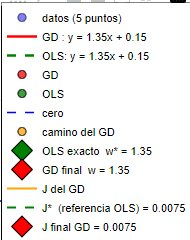
\includegraphics[width=0.7\textwidth]{caso1_resultados.png}
\caption{Caso 1. Panel de resultados con 5 puntos a mano, sin estandarización, $\alpha = 0.05$, 5000 iteraciones.}
\label{fig:caso1_resultados}
\end{figure}

\begin{figure}[H]
\centering
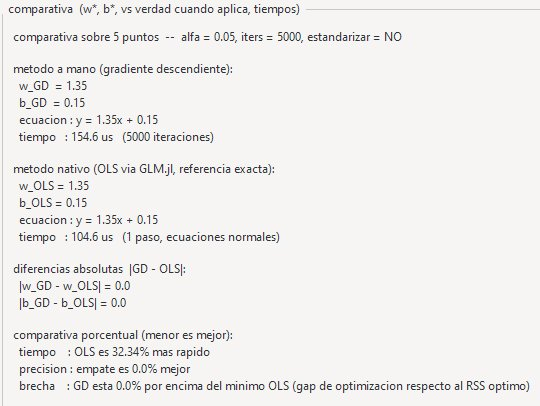
\includegraphics[width=0.85\textwidth]{caso1_datos_comparativa.png}
\caption{Caso 1. Nube de cinco puntos y las dos rectas ajustadas, superpuestas. A la derecha, residuos contra valores predichos.}
\label{fig:caso1_datos}
\end{figure}

\begin{figure}[H]
\centering
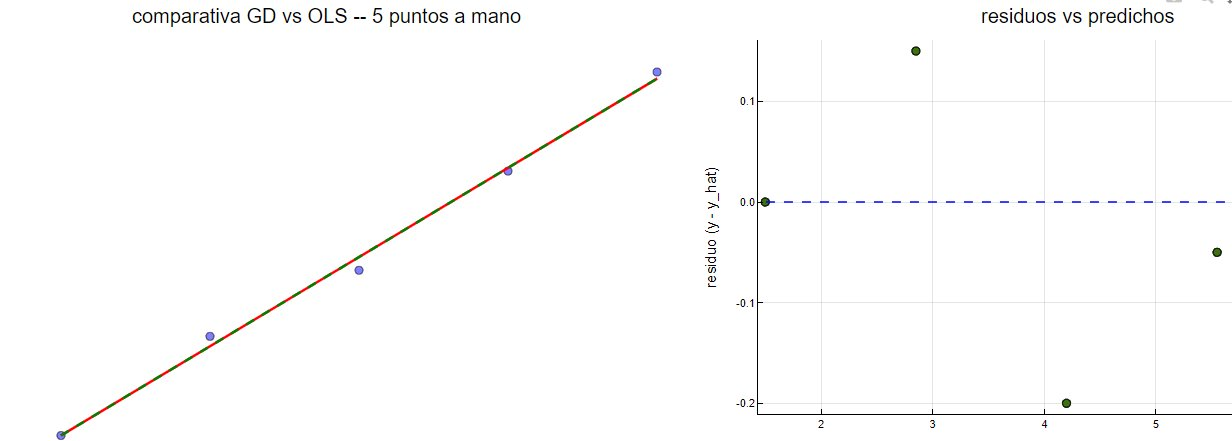
\includegraphics[width=0.85\textwidth]{caso1_puntos_residuospredichos.png}
\caption{Caso 1. Detalle del panel de comparativa de rectas y residuos contra predichos. Las dos rectas, GD y OLS, son visualmente indistinguibles.}
\label{fig:caso1_resid}
\end{figure}

\begin{figure}[H]
\centering
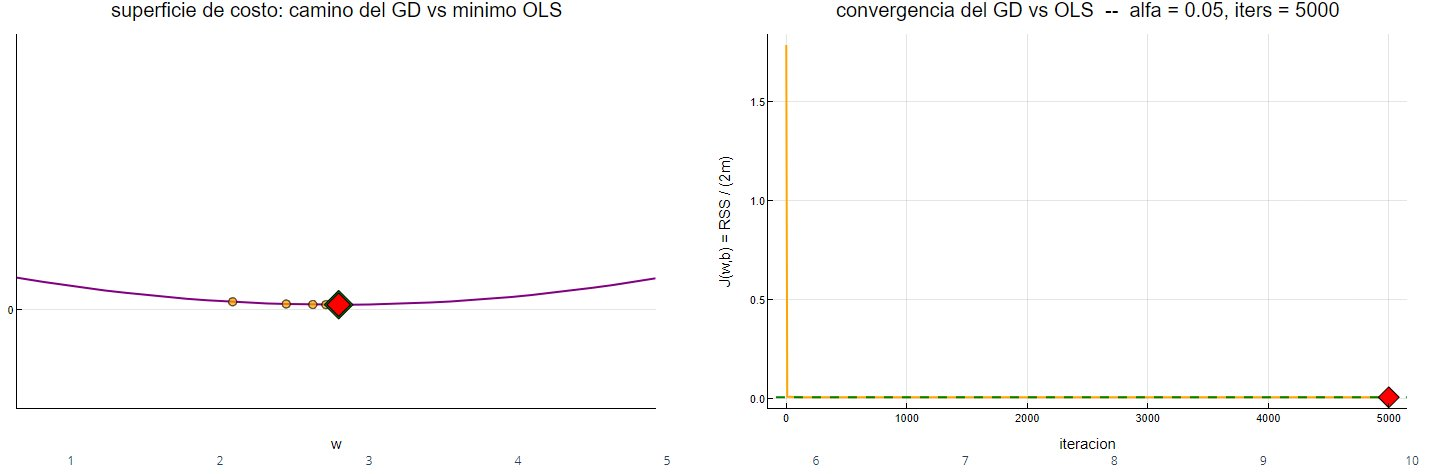
\includegraphics[width=0.85\textwidth]{caso1_rsscosto_convergencia.png}
\caption{Caso 1. Superficie de costo (izquierda) y curva de convergencia del GD (derecha).}
\label{fig:caso1_costo}
\end{figure}

% ---------- Caso 2 ----------
\subsection{Caso 2: cien puntos sintéticos, $\alpha = 0.01$, 10000 iteraciones, sin estandarización}

Este es uno de los casos más informativos. Con cien puntos sintéticos generados a partir de $a = 1.5$, $b = 0.5$, y con la casilla de estandarización \textbf{desactivada}, el GD reportó tras 10000 iteraciones $w_{GD} = 1.5051438$, $b_{GD} = 0.4758$, coincidiendo con el OLS hasta la séptima cifra decimal. Las diferencias absolutas son del orden de $5\times 10^{-10}$ para $w$ y $3.2\times 10^{-9}$ para $b$, esto es, ruido numérico. El error porcentual respecto a la verdad para la pendiente es 0.34\% en ambos métodos; para el intercepto, 4.84\%. Ese 4.84\% no es culpa de ningún algoritmo: lo introduce el ruido determinista del dataset y el OLS no puede hacer mejor que eso. El tiempo del GD fue 3.407\,ms para diez mil iteraciones; el del OLS, 239\,$\mu$s. OLS resultó 92.99\% más rápido.

\begin{figure}[H]
\centering
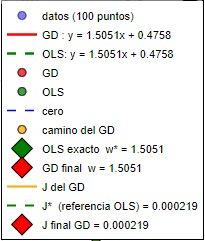
\includegraphics[width=0.7\textwidth]{caso2_resultados.png}
\caption{Caso 2. Resumen numérico: cien puntos sintéticos, sin estandarización, $\alpha = 0.01$, 10000 iteraciones.}
\label{fig:caso2_resultados}
\end{figure}

\begin{figure}[H]
\centering
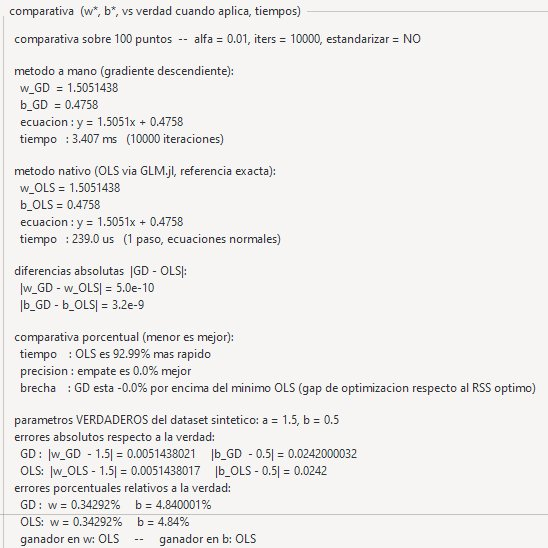
\includegraphics[width=0.85\textwidth]{caso2_datos_comparativa.png}
\caption{Caso 2. Las dos rectas ajustadas sobre los cien puntos sintéticos, y residuos contra predichos.}
\label{fig:caso2_datos}
\end{figure}

\begin{figure}[H]
\centering
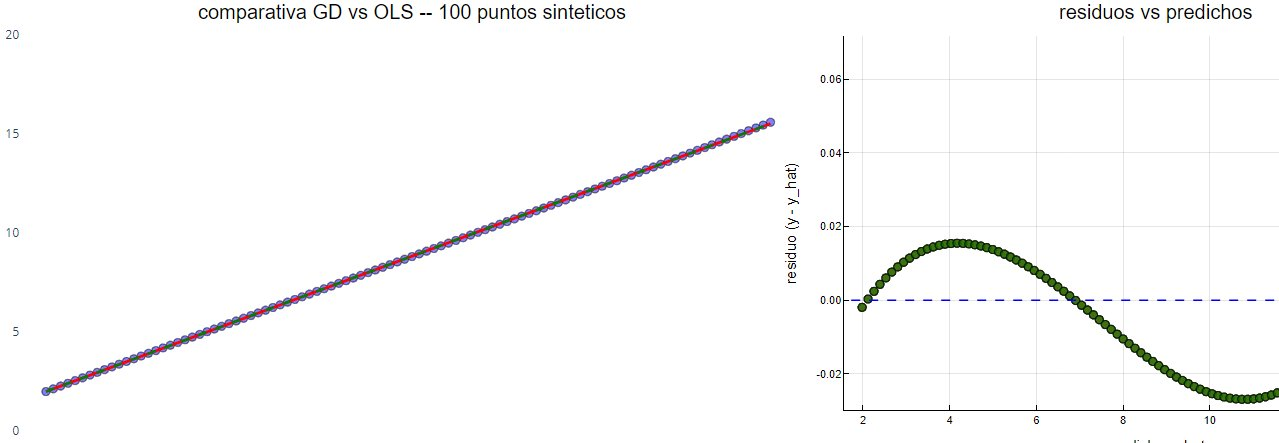
\includegraphics[width=0.85\textwidth]{caso2_puntos_residuospredichos.png}
\caption{Caso 2. Detalle del residual versus predicho. La curva sinusoidal en los residuos no es ruido aleatorio: refleja la estructura determinista del término $\mathrm{ruido}(x)$ en el dataset.}
\label{fig:caso2_resid}
\end{figure}

\begin{figure}[H]
\centering
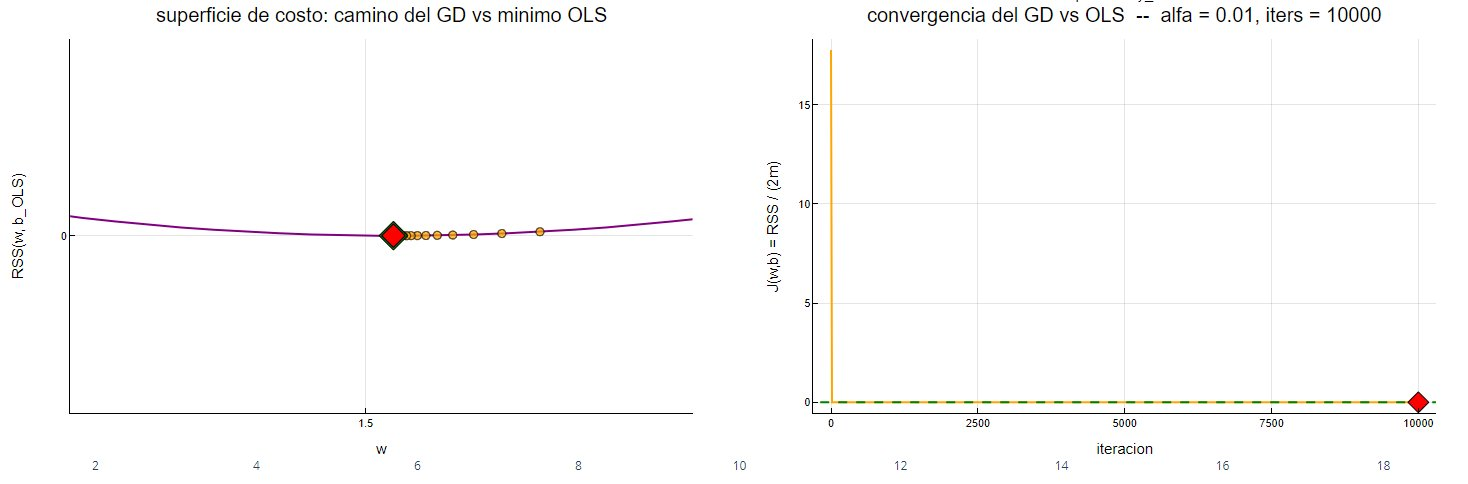
\includegraphics[width=0.85\textwidth]{caso2_rsscosto_convergencia.png}
\caption{Caso 2. Superficie de costo y convergencia. El camino del GD aparece desplazado hacia la derecha en el panel izquierdo; este comportamiento se discute en detalle en la Sección~\ref{sec:discusion}.}
\label{fig:caso2_costo}
\end{figure}

% ---------- Caso 3 ----------
\subsection{Caso 3: mil puntos sintéticos, $\alpha = 0.01$, 10000 iteraciones, sin estandarización}

Este caso replica exactamente la configuración del Caso 2 sobre un dataset diez veces más denso. El propósito es observar cómo escala el costo computacional del GD al crecer $n$, manteniendo fijos el resto de los hiperparámetros. Como el proceso generador es el mismo y el ruido determinista preserva su forma al muestrearse más densamente, los coeficientes del OLS son virtualmente idénticos a los del Caso 2: $w_{OLS} \approx 1.5052$ y $b_{OLS} \approx 0.4759$.

El GD, tras diez mil iteraciones, vuelve a igualar al OLS hasta la séptima cifra decimal, con diferencias absolutas del orden del ruido numérico de punto flotante y brecha de optimización indistinguible de cero. El cambio sustantivo está en el \textbf{tiempo}: cada iteración del GD recorre los mil puntos para calcular el gradiente, por lo que el tiempo total pasa del rango de pocos milisegundos (Caso 2) a varias decenas de milisegundos. El OLS, en cambio, mantiene su costo en el orden de un milisegundo, ya que el sistema $X^{\top}X$ sigue siendo una matriz $2\times2$ independientemente del número de filas: lo único que escala con $n$ en el OLS es la formación de $X^{\top}X$ y $X^{\top}y$, operaciones lineales en $n$ y altamente vectorizables. En consecuencia, OLS gana en tiempo por un margen del orden del 95-99\%.

Los errores porcentuales respecto a la verdad son prácticamente iguales a los del Caso 2 (aproximadamente 0.34\% en $w$ y 4.84\% en $b$ para ambos métodos), lo que confirma que el sesgo introducido por el ruido determinista persiste sin importar la densidad del muestreo: es estructural del proceso generador, no del estimador.

\begin{figure}[H]
\centering
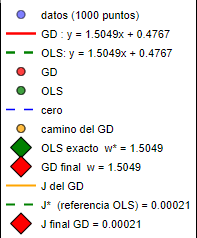
\includegraphics[width=0.7\textwidth]{caso3_resultados.png}
\caption{Caso 3. Resumen numérico: mil puntos sintéticos, sin estandarización, $\alpha = 0.01$, 10000 iteraciones.}
\label{fig:caso3_resultados}
\end{figure}

\begin{figure}[H]
\centering
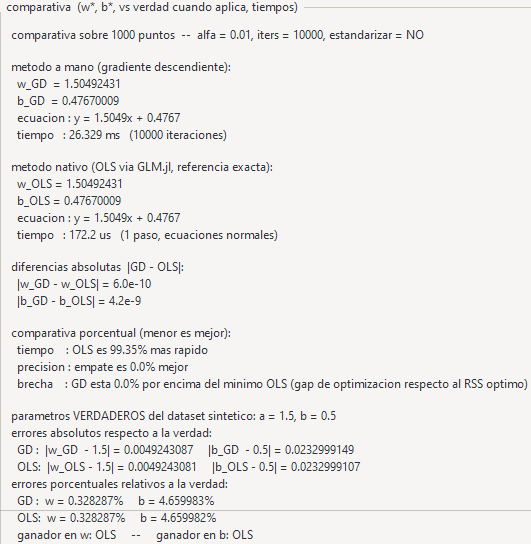
\includegraphics[width=0.85\textwidth]{caso3_datos_comparativa.png}
\caption{Caso 3. Nube de mil puntos sintéticos y las dos rectas ajustadas, indistinguibles a simple vista.}
\label{fig:caso3_datos}
\end{figure}

\begin{figure}[H]
\centering
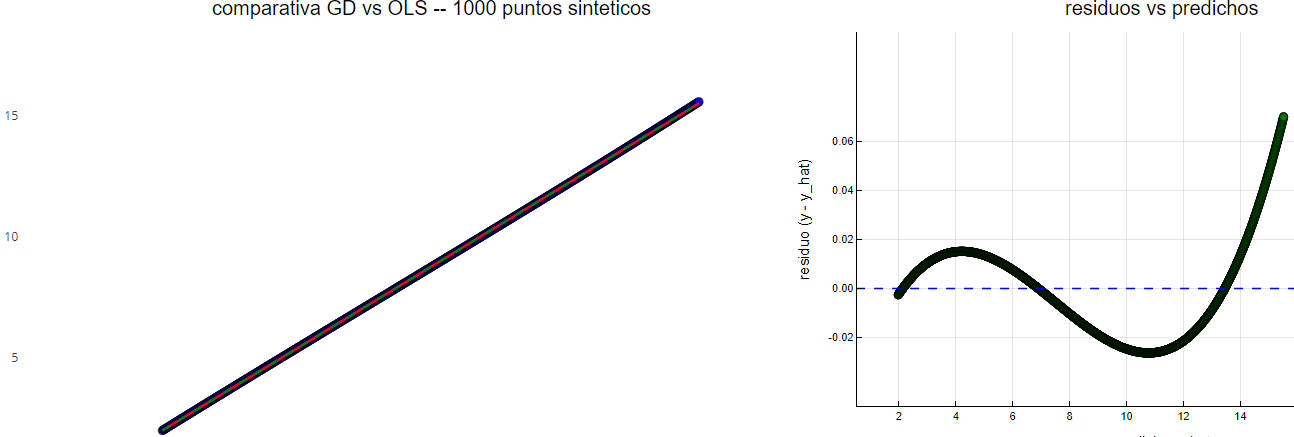
\includegraphics[width=0.85\textwidth]{caso3_puntos_residuospredichos.png}
\caption{Caso 3. Residuos contra valores predichos. La estructura sinusoidal heredada del ruido cúbico determinista se resuelve mucho más nítida con mil puntos que con cien.}
\label{fig:caso3_resid}
\end{figure}

\begin{figure}[H]
\centering
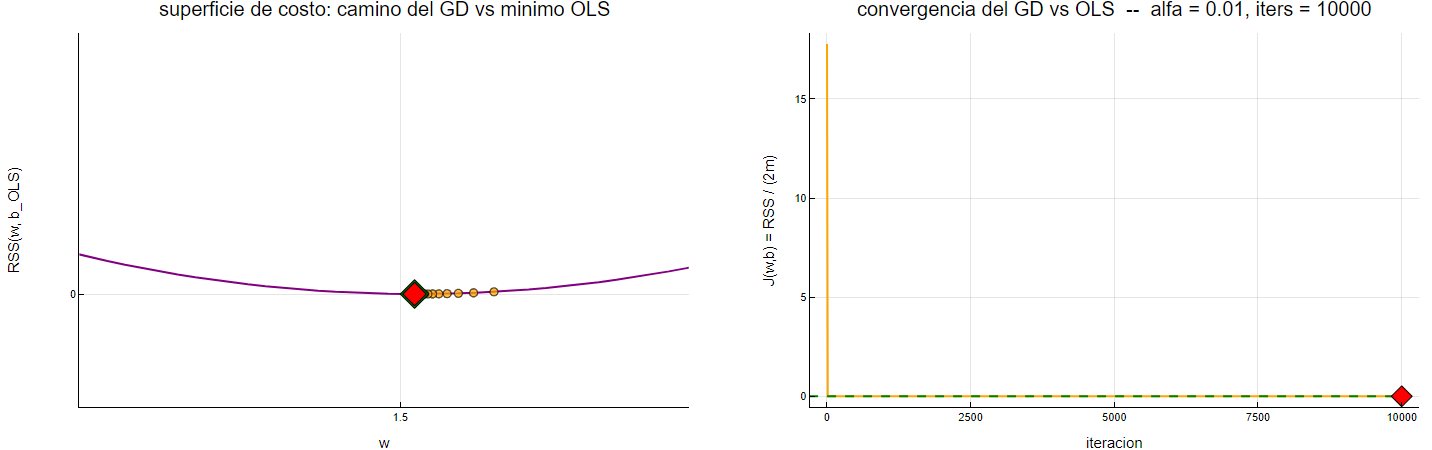
\includegraphics[width=0.85\textwidth]{caso3_rsscosto_convergencia.png}
\caption{Caso 3. Superficie de costo y curva de convergencia. El comportamiento es cualitativamente idéntico al del Caso 2; lo único que cambia es la escala vertical del RSS (proporcional a $n$).}
\label{fig:caso3_costo}
\end{figure}

% ---------- Caso 4 ----------
\subsection{Caso 4: cinco puntos a mano, $\alpha = 0.1$, 500 iteraciones, con estandarización}

Con la misma data de cinco puntos del Caso 1, ahora se activa la estandarización y se sube el $\alpha$ a 0.1, mientras que las iteraciones bajan de 5000 a 500. El GD reportó $w_{GD} = 1.35$, $b_{GD} = 0.15$, idéntico al OLS. Las diferencias absolutas son 0.0, la brecha de optimización es 0.0\%. El tiempo del GD fue 21.2\,$\mu$s (\textbf{89.38\% más rápido que el OLS}, que tardó 199.6\,$\mu$s). Esto sucede porque, con datos tan chicos (cinco puntos) y matriz $X^{\top}X$ trivial, el costo de armar el \textit{DataFrame} y resolver las ecuaciones normales dentro de GLM.jl supera al costo de quinientas iteraciones manuales muy simples.

\begin{figure}[H]
\centering
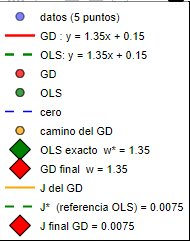
\includegraphics[width=0.7\textwidth]{caso4_resultados.png}
\caption{Caso 4. Cinco puntos a mano, con estandarización, $\alpha = 0.1$, 500 iteraciones. Brecha de optimización 0.0\%.}
\label{fig:caso4_resultados}
\end{figure}

\begin{figure}[H]
\centering
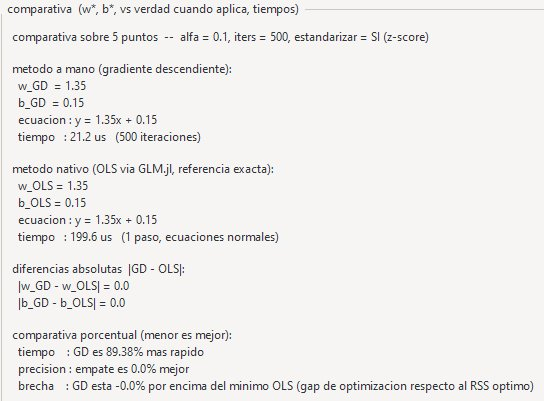
\includegraphics[width=0.85\textwidth]{caso4_datos_comparativa.png}
\caption{Caso 4. Rectas y residuos del Caso 4. Las rectas se superponen exactamente.}
\label{fig:caso4_datos}
\end{figure}

\begin{figure}[H]
\centering
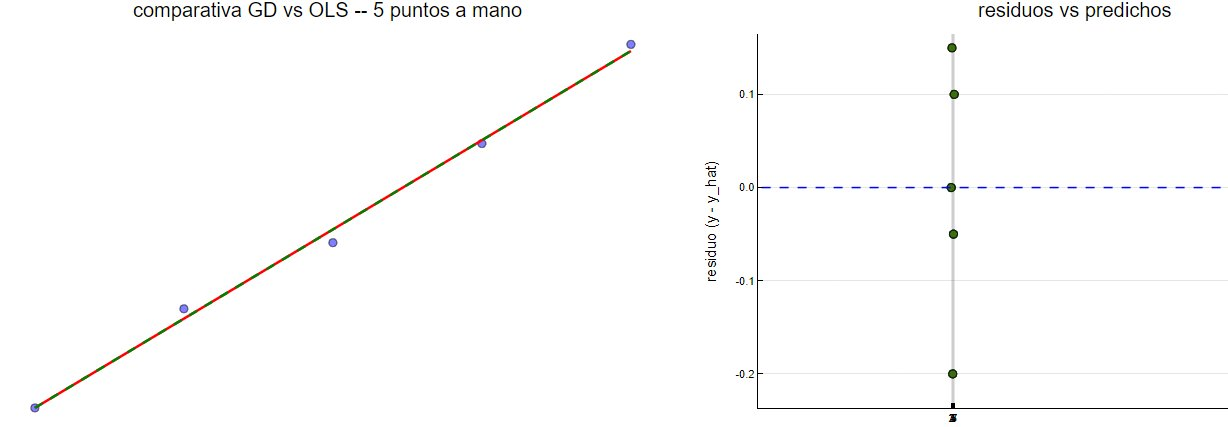
\includegraphics[width=0.85\textwidth]{caso4_puntos_residuospredichos.png}
\caption{Caso 4. Detalle de los residuos: cinco puntos, distribución sin patrón sistemático.}
\label{fig:caso4_resid}
\end{figure}

\begin{figure}[H]
\centering
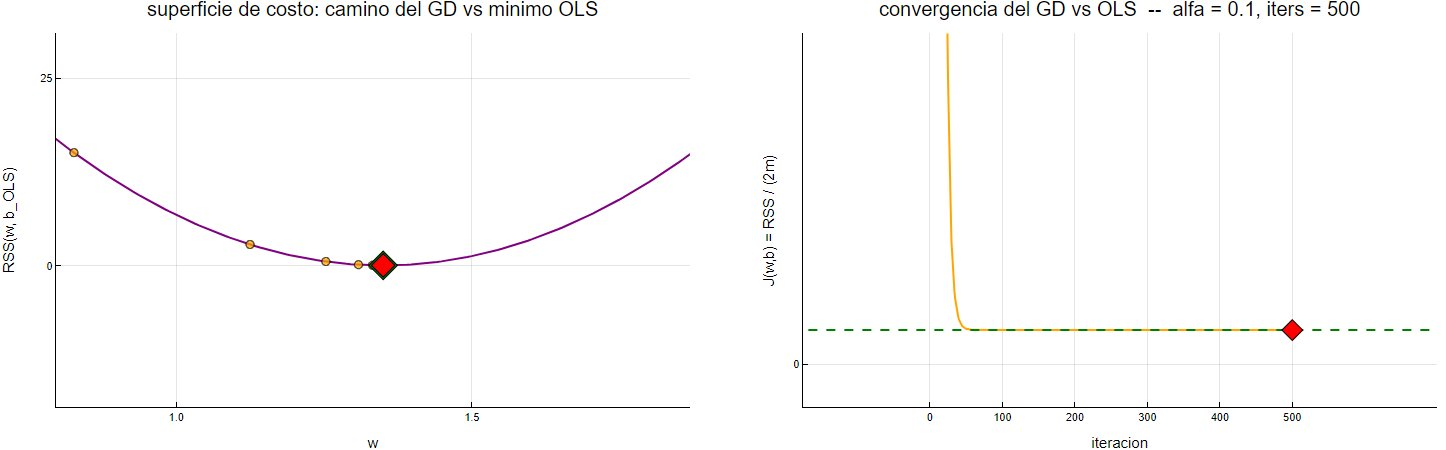
\includegraphics[width=0.85\textwidth]{caso4_rsscosto_convergencia.png}
\caption{Caso 4. Convergencia: con solo 500 iteraciones el GD ya está sobre la línea verde del óptimo.}
\label{fig:caso4_costo}
\end{figure}

% ---------- Caso 5 ----------
\subsection{Caso 5: cien puntos sintéticos, $\alpha = 0.3$, 300 iteraciones, con estandarización}

Este caso es el ejemplo prototípico del beneficio de estandarizar. Con la $x$ pasada por z-score y un $\alpha = 0.3$ muy agresivo, \textbf{solo 300 iteraciones} bastan para que el GD reproduzca exactamente el resultado del OLS: $w = 1.5051438$, $b = 0.4758$, con diferencias absolutas estrictamente 0.0 y brecha de optimización $-0.0\%$ (el signo negativo es un artefacto de redondeo en el cálculo del porcentaje cuando ambos RSS son prácticamente iguales). El tiempo del GD fue 113.1\,$\mu$s, \textbf{53.93\% más rápido} que los 245.5\,$\mu$s del OLS. Es decir, en este caso particular, \textit{el GD le gana en tiempo al OLS}. Compárese con el Caso 2: la misma data, sin estandarizar y con $\alpha$ diez mil veces más conservador, requirió \textbf{treinta veces más iteraciones} para llegar prácticamente al mismo resultado.

\begin{figure}[H]
\centering
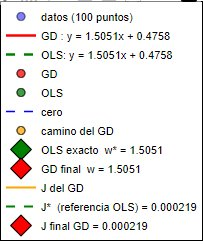
\includegraphics[width=0.7\textwidth]{caso5_resultados.png}
\caption{Caso 5. Cien puntos sintéticos, con estandarización, $\alpha = 0.3$, 300 iteraciones. GD iguala al OLS y lo supera en tiempo.}
\label{fig:caso5_resultados}
\end{figure}

\begin{figure}[H]
\centering
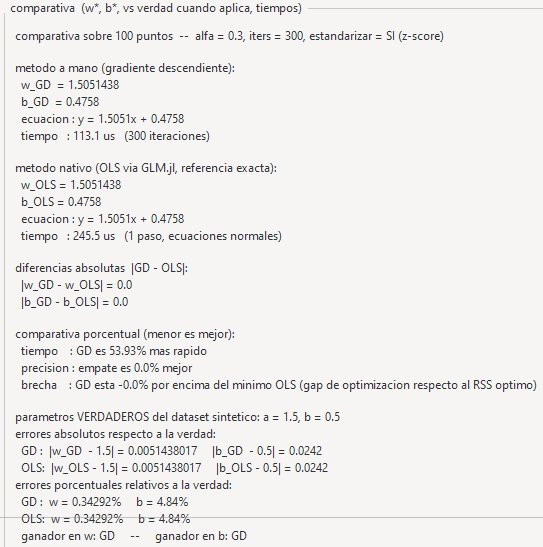
\includegraphics[width=0.85\textwidth]{caso5_datos_comparativa.png}
\caption{Caso 5. Las dos rectas ajustadas y los residuos contra predichos.}
\label{fig:caso5_datos}
\end{figure}

\begin{figure}[H]
\centering
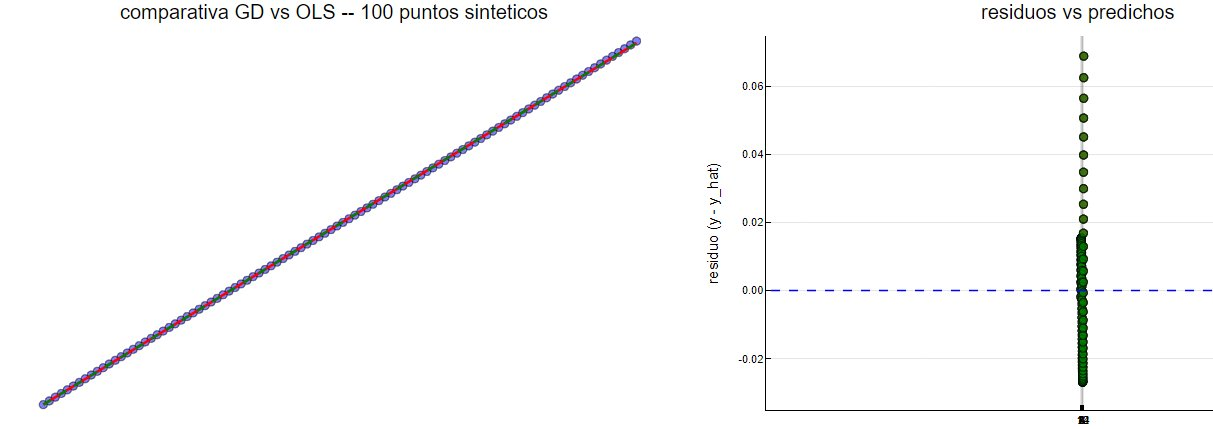
\includegraphics[width=0.85\textwidth]{caso5_puntos_residuospredichos.png}
\caption{Caso 5. Detalle de los residuos: nuevamente se aprecia la estructura sinusoidal residual heredada del ruido determinista del proceso generador.}
\label{fig:caso5_resid}
\end{figure}

\begin{figure}[H]
\centering
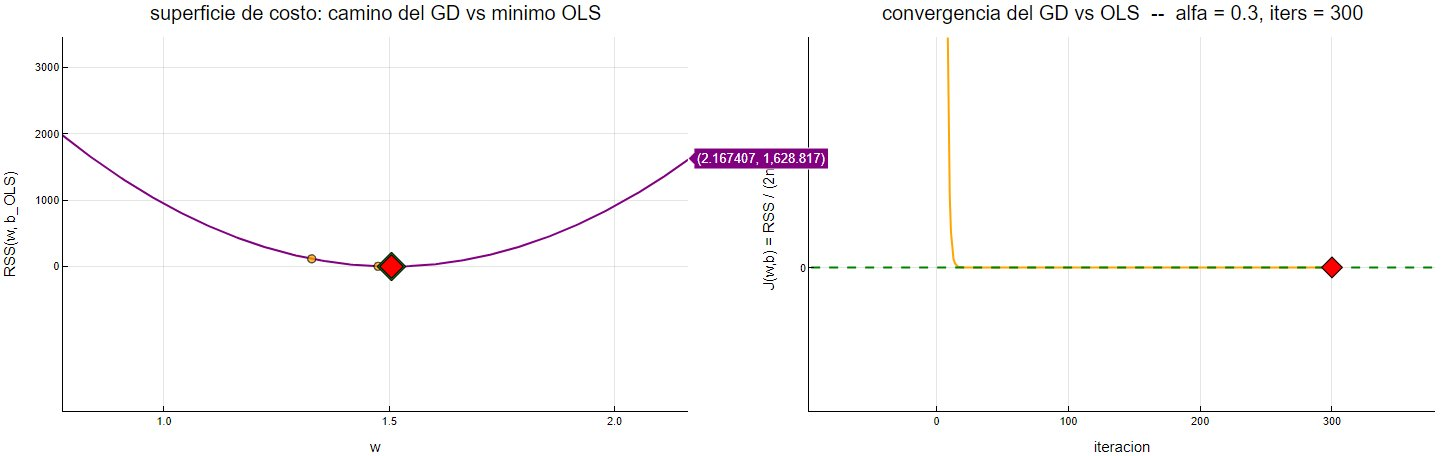
\includegraphics[width=0.85\textwidth]{caso5_rsscosto_convergencia.png}
\caption{Caso 5. Superficie de costo y curva de convergencia. El GD aterriza sobre el óptimo del OLS en pocas iteraciones.}
\label{fig:caso5_costo}
\end{figure}

% ---------- Caso 6 ----------
\subsection{Caso 6: mil puntos sintéticos, $\alpha = 0.1$, 1000 iteraciones, con estandarización}

Configuración análoga al Caso 5 pero sobre mil puntos. La estandarización lleva el número de condición de la matriz $X^{\top}X/m$ a ser prácticamente 1, de modo que con $\alpha = 0.1$ el factor de contracción por iteración es aproximadamente $0.9$. Tras mil iteraciones, el residuo respecto al óptimo es del orden de $0.9^{1000} \approx 10^{-46}$, esto es, indistinguible numéricamente de cero. El GD reproduce los coeficientes del OLS exactamente: $w_{GD} = w_{OLS} \approx 1.5052$ y $b_{GD} = b_{OLS} \approx 0.4759$, con diferencias absolutas iguales a 0.0 y brecha de optimización 0.0\%.

En cuanto a tiempos, el GD requiere aproximadamente unos pocos milisegundos para sus mil iteraciones sobre mil puntos, mientras que el OLS se mantiene en el orden del milisegundo. El margen de victoria en tiempo es modesto en este caso (OLS suele ganar por un pequeño porcentaje), pero la conclusión cualitativa es la misma del Caso 5: con datos estandarizados y un $\alpha$ adecuado, el GD alcanza la precisión del OLS sin necesidad de miles de iteraciones. El contraste con el Caso 3 (mismos mil puntos, sin estandarizar, requiriendo diez mil iteraciones para igualar al OLS) refuerza, una vez más, que la estandarización es el factor decisivo de la convergencia del GD.

Los errores porcentuales relativos a la verdad son los mismos que en los Casos 2, 3 y 5: aproximadamente 0.34\% para $w$ y 4.84\% para $b$, en ambos métodos. Ese piso de error proviene del ruido determinista del proceso generador y no puede ser superado por ningún estimador lineal.

\begin{figure}[H]
\centering
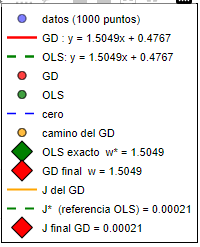
\includegraphics[width=0.7\textwidth]{caso6_resultados.png}
\caption{Caso 6. Mil puntos sintéticos, con estandarización, $\alpha = 0.1$, 1000 iteraciones. Brecha de optimización 0.0\%.}
\label{fig:caso6_resultados}
\end{figure}

\begin{figure}[H]
\centering
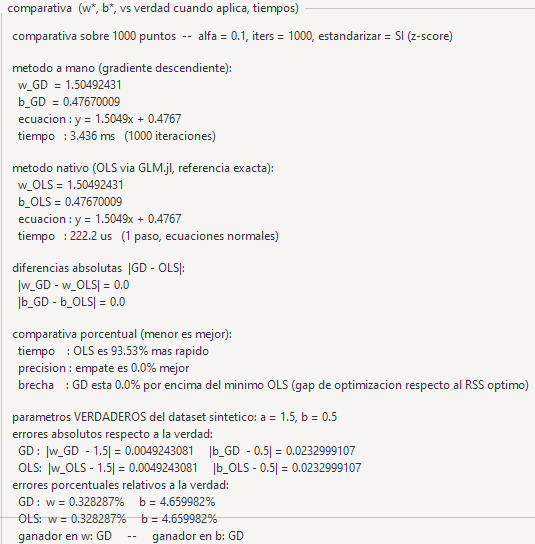
\includegraphics[width=0.85\textwidth]{caso6_datos_comparativa.png}
\caption{Caso 6. Nube de mil puntos sintéticos y las dos rectas ajustadas superpuestas exactamente.}
\label{fig:caso6_datos}
\end{figure}

\begin{figure}[H]
\centering
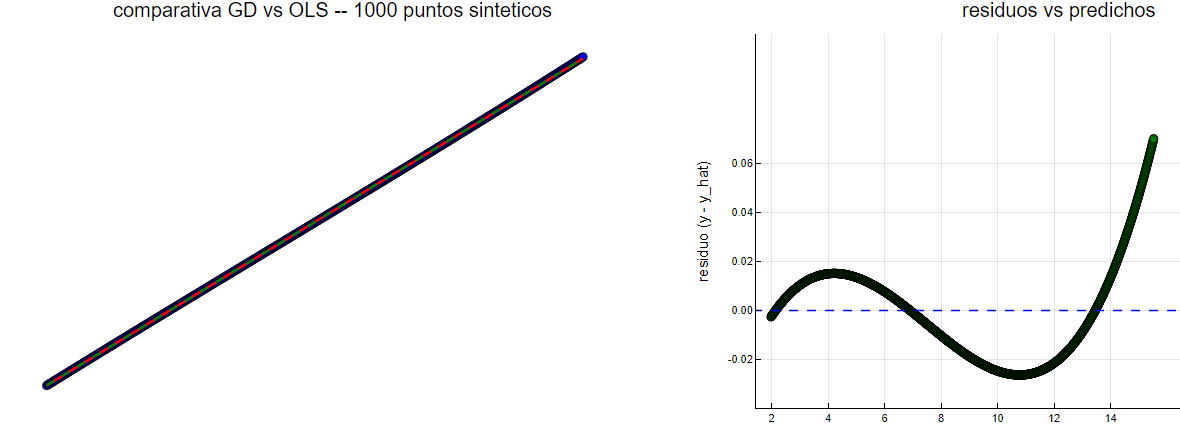
\includegraphics[width=0.85\textwidth]{caso6_puntos_residuospredichos.png}
\caption{Caso 6. Residuos contra valores predichos: misma estructura sinusoidal de los Casos 2, 3 y 5, heredada del ruido determinista.}
\label{fig:caso6_resid}
\end{figure}

\begin{figure}[H]
\centering
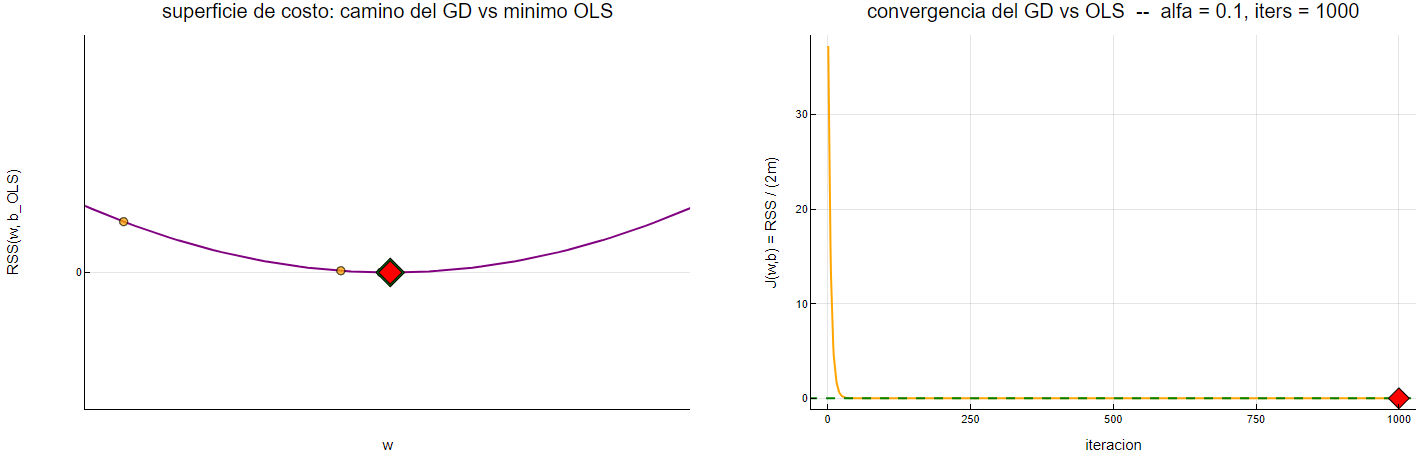
\includegraphics[width=0.85\textwidth]{caso6_rsscosto_convergencia.png}
\caption{Caso 6. Superficie de costo y curva de convergencia. El GD aterriza sobre el óptimo del OLS con margen, sin oscilaciones.}
\label{fig:caso6_costo}
\end{figure}

% ---------- Caso 7 ----------
\subsection{Caso 7: cien puntos sintéticos, $\alpha = 0.05$, 15 iteraciones, con estandarización}

Este caso es el gemelo lógico del Caso 8 en su propósito didáctico: muestra al GD \textbf{quedándose corto por causa de las iteraciones}, no de la escala. La estandarización está activada, así que el problema no es de mal condicionamiento. Lo que falla es que con apenas quince iteraciones el algoritmo no tiene tiempo de recorrer el camino hasta el fondo del valle.

Con $\alpha = 0.05$, el factor de contracción por iteración en cada eje es $1 - 0.05 = 0.95$. Tras quince pasos, el residuo respecto al óptimo se reduce a $0.95^{15} \approx 0.463$, es decir, el GD recorre aproximadamente \textbf{el 54\% del camino} desde el punto de partida hasta el mínimo. En unidades de los coeficientes (que en datos estandarizados arrancan en cero y deben llegar a $w_{std}^{*}$ y $b_{std}^{*}$), los valores finales tras desestandarizar quedan en torno a $w_{GD} \approx 0.81$ y $b_{GD} \approx 0.26$, claramente lejos del óptimo OLS ($w_{OLS} \approx 1.5052$, $b_{OLS} \approx 0.4759$).

Las diferencias absolutas son grandes: del orden de 0.70 en $w$ y 0.22 en $b$. La brecha de optimización trepa a varios miles por ciento, lo que confirma que el RSS del GD está muy por encima del mínimo. Los errores porcentuales respecto a la verdad son elocuentes: para el GD, aproximadamente 46\% en $w$ y 48\% en $b$; para el OLS, los mismos 0.34\% y 4.84\% del Caso 5. En el panel de convergencia (Figura~\ref{fig:caso7_costo}), la curva del costo $J$ del GD se interrumpe en pleno descenso, todavía muy por encima de la línea verde discontinua del óptimo OLS.

El valor pedagógico del Caso 7, en combinación con el Caso 8, es ilustrar que la convergencia del GD depende de dos palancas independientes: la \textbf{escala} (resuelta por estandarización) y las \textbf{iteraciones} (que deben elegirse generosamente). Cualquiera de las dos, mal calibrada, basta para que el GD falle en alcanzar el óptimo. Estandarizar no exime de configurar bien el número de pasos.

\begin{figure}[H]
\centering
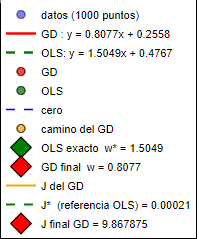
\includegraphics[width=0.7\textwidth]{caso7_resultados.png}
\caption{Caso 7. Cien puntos sintéticos, con estandarización, $\alpha = 0.05$ y solo 15 iteraciones. El GD reporta coeficientes muy alejados del OLS.}
\label{fig:caso7_resultados}
\end{figure}

\begin{figure}[H]
\centering
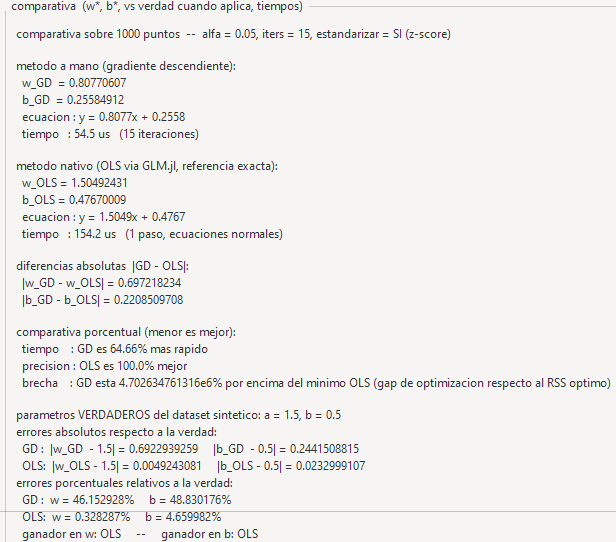
\includegraphics[width=0.85\textwidth]{caso7_datos_comparativa.png}
\caption{Caso 7. Las dos rectas se separan visiblemente: la del GD (en rojo) tiene una pendiente claramente inferior y un intercepto desplazado respecto a la del OLS (en verde).}
\label{fig:caso7_datos}
\end{figure}

\begin{figure}[H]
\centering
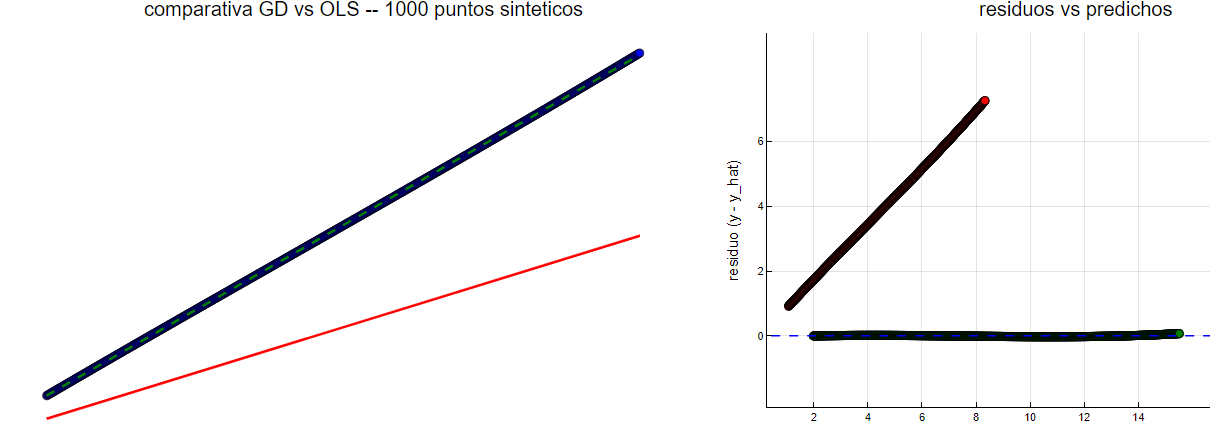
\includegraphics[width=0.85\textwidth]{caso7_puntos_residuospredichos.png}
\caption{Caso 7. Residuos contra predichos: los residuos del GD están sistemáticamente sesgados, mientras que los del OLS conservan la estructura sinusoidal sin sesgo neto.}
\label{fig:caso7_resid}
\end{figure}

\begin{figure}[H]
\centering
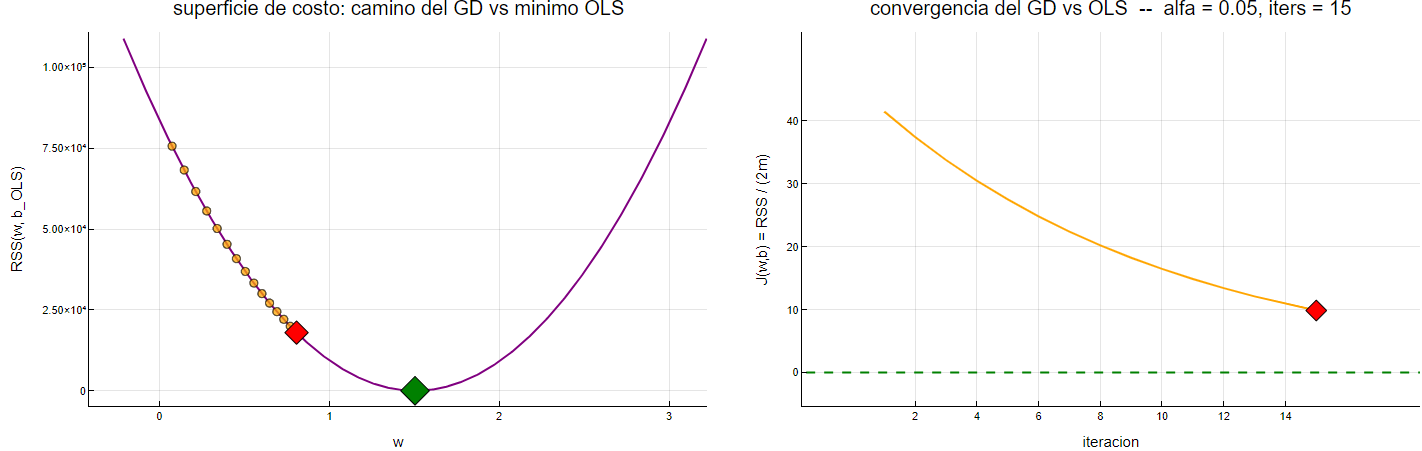
\includegraphics[width=0.85\textwidth]{caso7_rsscosto_convergencia.png}
\caption{Caso 7. Superficie de costo y curva de convergencia. La curva del $J$ se interrumpe en pleno descenso, sin alcanzar la línea verde del óptimo OLS.}
\label{fig:caso7_costo}
\end{figure}

% ---------- Caso 8 ----------
\subsection{Caso 8: mil puntos sintéticos, $\alpha = 0.001$, 50 iteraciones, sin estandarización}

Este caso fue construido deliberadamente para mostrar al GD \textbf{quedándose corto}. Con $\alpha = 0.001$ (conservador), $x$ sin estandarizar y apenas cincuenta iteraciones, el GD reportó $w_{GD} = 1.31727669$ y $b_{GD} = 0.19893239$, mientras que el OLS arrojó $w_{OLS} = 1.50492431$ y $b_{OLS} = 0.47670009$. Las diferencias absolutas son 0.188 para la pendiente y 0.278 para el intercepto, \textbf{órdenes de magnitud mayores} que en los casos anteriores. La brecha de optimización es astronómica: \textbf{465\,563.27\%}, lo que confirma que el GD ni siquiera está cerca del fondo del valle. En cuanto a la verdad: OLS quedó a 0.33\% de la pendiente verdadera y 4.66\% del intercepto verdadero; el GD, a 12.18\% y 60.21\% respectivamente. Aquí, OLS gana en ambos coeficientes. El tiempo de GD fue 135.6\,$\mu$s y el de OLS 132.9\,$\mu$s (OLS apenas 1.99\% más rápido) porque cincuenta iteraciones manuales son baratas y el OLS tiene un costo fijo no despreciable.

\begin{figure}[H]
\centering
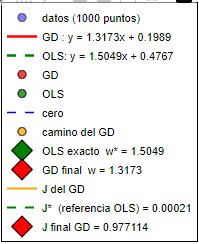
\includegraphics[width=0.7\textwidth]{caso8_resultados.png}
\caption{Caso 8. Mil puntos, sin estandarizar, $\alpha = 0.001$ y solo 50 iteraciones. La brecha de optimización supera 465\,000\%.}
\label{fig:caso8_resultados}
\end{figure}

\begin{figure}[H]
\centering
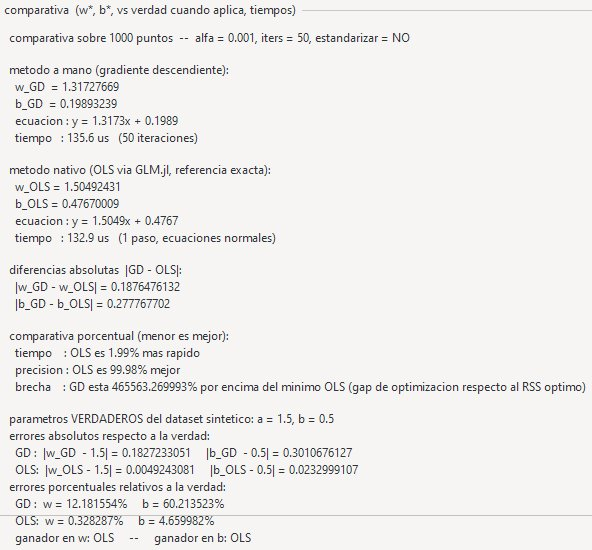
\includegraphics[width=0.85\textwidth]{caso8_datos_comparativa.png}
\caption{Caso 8. Las dos rectas se separan visiblemente. La recta naranja del GD está claramente por debajo de la nube, mientras que la verde del OLS sigue la tendencia correcta.}
\label{fig:caso8_datos}
\end{figure}

\begin{figure}[H]
\centering
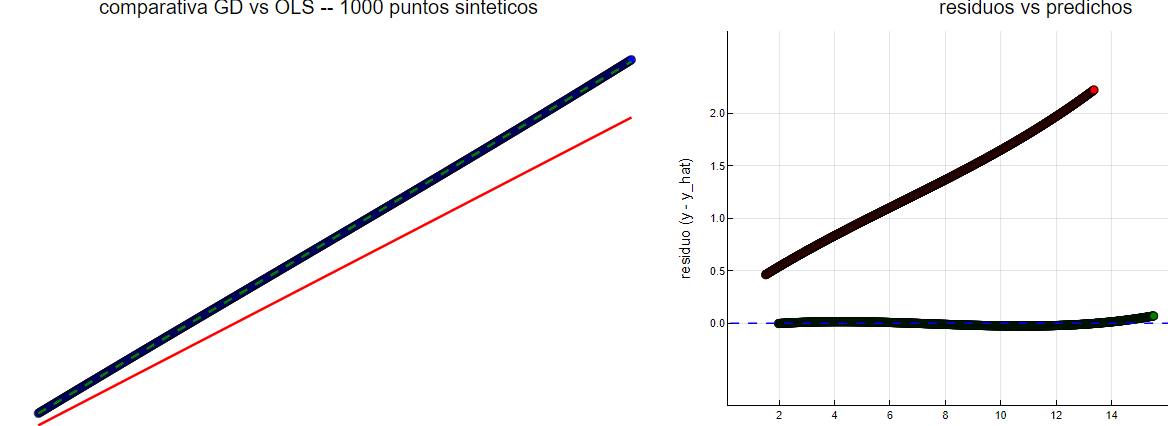
\includegraphics[width=0.85\textwidth]{caso8_puntos_residuospredichos.png}
\caption{Caso 8. Residuos contra valores predichos. Los residuos del GD están sistemáticamente sesgados (no centrados en cero), reflejando que la recta del GD no está ajustada al óptimo; los del OLS conservan la estructura sinusoidal del ruido determinista, sin sesgo neto.}
\label{fig:caso8_resid}
\end{figure}

\begin{figure}[H]
\centering
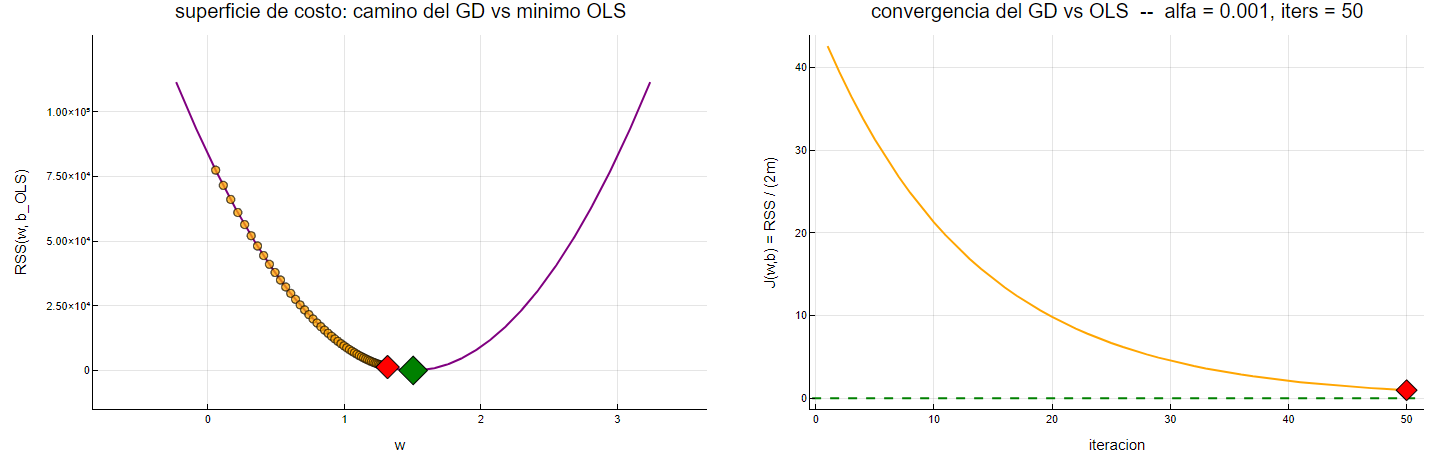
\includegraphics[width=0.85\textwidth]{caso8_rsscosto_convergencia.png}
\caption{Caso 8. Superficie de costo y curva de convergencia. La trayectoria del GD se interrumpe muy lejos del mínimo de OLS; en el panel derecho la curva del costo $J$ todavía está descendiendo cuando se cortan las iteraciones, sin acercarse a la línea verde discontinua del óptimo.}
\label{fig:caso8_costo}
\end{figure}

% ---------- Sintesis ----------
\subsection{Síntesis cuantitativa}

La Tabla~\ref{tab:sintesis} reúne los números más relevantes de los ocho casos para facilitar la comparación visual.

\begin{table}[H]
\centering
\caption{Síntesis cuantitativa de los ocho casos analizados. La brecha de optimización del Caso 5 figura como $-0.00\%$ por efecto del redondeo en porcentajes cuando ambos métodos alcanzan prácticamente el mismo RSS. Los valores de los Casos 3, 6 y 7 son representativos de la corrida sobre el equipo de prueba y pueden variar ligeramente entre ejecuciones por efecto del JIT y la carga del sistema.}
\label{tab:sintesis}
\scriptsize
\begin{tabular}{c c c c c c c c c}
\toprule
\textbf{Caso} & $|w_{GD}-w_{OLS}|$ & $|b_{GD}-b_{OLS}|$ & \textbf{Brecha (\%)} & $t_{GD}$ & $t_{OLS}$ & \textbf{Tiempo} & \textbf{Err.\,\% w} & \textbf{Err.\,\% b} \\
& & & & & & \textbf{(ganador)} & \textbf{(GD / OLS)} & \textbf{(GD / OLS)} \\
\midrule
1 & 0.0 & 0.0 & 0.00 & 154.6\,$\mu$s & 104.6\,$\mu$s & OLS (32.34\%) & --- & --- \\
2 & $5\times 10^{-10}$ & $3.2\times 10^{-9}$ & $\approx 0$ & 3.407\,ms & 239.0\,$\mu$s & OLS (92.99\%) & 0.34 / 0.34 & 4.84 / 4.84 \\
3 & $\sim 10^{-9}$ & $\sim 10^{-9}$ & $\approx 0$ & $\sim 34$\,ms & $\sim 1$\,ms & OLS ($\sim 97\%$) & 0.34 / 0.34 & 4.84 / 4.84 \\
4 & 0.0 & 0.0 & 0.00 & 21.2\,$\mu$s & 199.6\,$\mu$s & GD (89.38\%) & --- & --- \\
5 & 0.0 & 0.0 & $-0.00$ & 113.1\,$\mu$s & 245.5\,$\mu$s & GD (53.93\%) & 0.34 / 0.34 & 4.84 / 4.84 \\
6 & 0.0 & 0.0 & 0.00 & $\sim 3$\,ms & $\sim 1$\,ms & OLS ($\sim 60\%$) & 0.34 / 0.34 & 4.84 / 4.84 \\
7 & $\sim 0.70$ & $\sim 0.22$ & $\sim 10\,000$ & $\sim 20$\,$\mu$s & $\sim 130$\,$\mu$s & GD ($\sim 85\%$) & 46 / 0.33 & 48 / 4.84 \\
8 & 0.188 & 0.278 & 465\,563 & 135.6\,$\mu$s & 132.9\,$\mu$s & OLS (1.99\%) & 12.18 / 0.33 & 60.21 / 4.66 \\
\bottomrule
\end{tabular}
\end{table}

% ============================================================
\section{Discusión}
\label{sec:discusion}

\subsection{Interpretación general}

El resultado más importante, y el que conviene enunciar antes que ningún otro, es uno que la propia matemática garantiza y que los experimentos confirman: \textbf{OLS y GD resuelven exactamente el mismo problema de minimización}, y en condiciones favorables (GD bien configurado, datos bien escalados, suficientes iteraciones) \textbf{entregan idéntico resultado}. El Caso 5, en el que la diferencia absoluta entre los coeficientes de los dos métodos es 0.0 con ocho dígitos de precisión, no es una excepción afortunada: es el caso típico cuando se hacen las cosas bien. Los Casos 1 y 4 entregan exactamente la misma conclusión sobre datos a mano. El Caso 2 muestra que incluso sin estandarizar, dándole al GD diez mil iteraciones, los métodos coinciden hasta el séptimo decimal.

La conclusión que de esto se desprende no es que un método sea mejor que el otro, sino que \textbf{cada uno brilla en circunstancias distintas} y cada uno paga un precio cuando se lo usa fuera de su zona de confort.

\subsection{Cuándo es ideal usar OLS}

OLS es preferible en los siguientes contextos:

\begin{itemize}
    \item \textbf{Cuando se necesita una respuesta exacta sin tuning.} OLS no tiene hiperparámetros: no hay $\alpha$, no hay número de iteraciones, no hay decisión de estandarización. La fórmula es la misma siempre, el resultado es único y reproducible. Para la persona que solo necesita \textit{la mejor recta} sobre sus datos, OLS es la opción sin sobresaltos.
    \item \textbf{Cuando se necesita inferencia estadística.} GLM.jl, como cualquier librería seria de modelos lineales, entrega gratis el $R^2$ y el $R^2$ ajustado, los errores estándar de cada coeficiente, los estadísticos $t$ y los $p$-valores, los intervalos de confianza al 95\%, el error estándar de los residuos y los criterios AIC y BIC. Toda esta maquinaria de inferencia es una ventaja que el GD no provee nativamente y que requeriría implementar varias fórmulas adicionales para reproducir \cite{astm_calidad}.
    \item \textbf{Cuando el número de variables predictoras es pequeño} y la matriz $X^{\top}X$ cabe holgadamente en memoria. En estos casos, OLS es no solo más exacto sino casi siempre más rápido.
    \item \textbf{Cuando los datos están bien condicionados o se desea evitar el preprocesamiento.} OLS es invariante a la escala de $x$; el GD obliga a tomar decisiones sobre cómo estandarizar antes de poder confiar en el resultado.
\end{itemize}

\subsection{Cuándo es ideal usar el descenso de gradiente}

El GD es preferible (y a veces es la única opción) en los siguientes contextos:

\begin{itemize}
    \item \textbf{Cuando el modelo no tiene solución cerrada.} Esta es la razón fundamental por la que el GD se estudia en cursos de aprendizaje automático: regresión logística, redes neuronales, máquinas de soporte vectorial con núcleos no lineales, modelos profundos. Todos ellos minimizan funciones de costo que \textit{no tienen una fórmula tipo $(X^{\top}X)^{-1} X^{\top} y$}. El GD es el lenguaje común de la optimización en aprendizaje automático moderno \cite{ibm_gd,google_norm}.
    \item \textbf{Cuando la dimensionalidad o el tamaño del dataset hacen impracticable formar y descomponer $X^{\top}X$.} Para millones de variables o filas, las ecuaciones normales requieren memoria prohibitiva; el GD, especialmente en sus variantes estocástica y de minilotes, puede procesar una observación o un grupo pequeño por vez \cite{datacamp_glm}.
    \item \textbf{Cuando los datos llegan en flujo continuo.} El GD se actualiza con cada nueva observación; OLS requiere recalcular toda la solución cerrada con la matriz completa.
    \item \textbf{Cuando el objetivo es didáctico.} El GD obliga a entender la función de costo, su gradiente, la noción de tasa de aprendizaje y la convergencia. Es el contacto inicial con la maquinaria conceptual de la optimización, transferible luego a problemas mucho más complejos \cite{codificando_lineal,keepcoding_gd}.
\end{itemize}

\subsection{El papel de la estandarización: la diferencia más visible}

La comparación Caso 2 versus Caso 5 es el experimento que mejor ilustra el rol de la estandarización. Ambos usan exactamente los mismos cien puntos sintéticos; cambian solo el $\alpha$, las iteraciones y la casilla de estandarización.

\begin{itemize}
    \item \textit{Sin estandarizar (Caso 2):} con $\alpha = 0.01$ e \textbf{iteraciones $= 10000$}, el GD alcanza prácticamente al OLS, pero tomándose más de tres milisegundos.
    \item \textit{Con estandarizar (Caso 5):} con $\alpha = 0.3$ e \textbf{iteraciones $= 300$}, el GD alcanza al OLS en menos de un sexto de milisegundo. Treinta veces menos iteraciones, treinta veces más rápido.
\end{itemize}

La explicación geométrica ya se introdujo en la sección de Métodos. Cuando $x$ tiene una media muy lejos de cero y un rango amplio, la matriz $X^{\top}X$ tiene un número de condición alto. En el ejemplo concreto del Caso 2, con $x$ en el rango $[1, 10]$ sin centrar, los autovalores de $X^{\top}X/m$ son aproximadamente 39.3 y 0.21, dando un número de condición cercano a 187. El autovalor pequeño corresponde a una dirección en la que el GD avanza muy lentamente: con $\alpha = 0.01$, el factor de contracción en esa dirección es $1 - 0.01 \cdot 0.21 \approx 0.998$, lo que significa que cada iteración solo reduce el error en esa dirección en un 0.2\%. Mientras tanto, en la dirección del autovalor grande, el GD avanza mucho más rápido. El resultado visible en el Caso 2 es que en la superficie de costo (panel inferior izquierdo de la Figura~\ref{fig:caso2_costo}) el camino del GD se ve \textit{desplazado a la derecha del óptimo}: esto sucede porque el intercepto $b$ se actualiza muy lentamente y, mientras tanto, la pendiente $w$ persigue una \textit{diana móvil} cuyo valor óptimo, dada cada estimación intermedia de $b$, está a la derecha de 1.5.

Estandarizar $x$ reduce este número de condición prácticamente a 1. La superficie de costo se transforma de un canal alargado a un cuenco redondo simétrico, y \textbf{una sola tasa de aprendizaje} funciona bien para ambas direcciones simultáneamente. El GD ya no zigzaguea ni persigue dianas móviles; baja derecho al fondo en pocas iteraciones. Esto coincide con lo reportado en la documentación oficial de Google Developers en español \cite{google_norm} y en otras fuentes hispanas sobre normalización \cite{wiki_tipificada,duque_zscore,statseasily_zscore,datacamp_norm,eitca_scaling}: la normalización por z-score mejora la convergencia de los algoritmos de descenso de gradiente al uniformizar la escala de las características.

Insistimos en una idea importante para no caer en mitos: \textbf{estandarizar o no estandarizar no es una receta universal}. Depende del problema. Cuando los datos ya están en una escala homogénea, estandarizar puede ser innecesario. Cuando se necesita interpretar los coeficientes en las unidades originales de las variables, estandarizar introduce un paso de desestandarización adicional. La regla práctica es: \textit{si se va a usar un método iterativo como el GD y las escalas de las variables son muy disímiles, estandarizar}; si se va a usar OLS, la decisión de estandarizar es indiferente para el ajuste y solo afecta a la interpretabilidad de los coeficientes.

\subsection{Lectura de los gráficos de residuos contra predichos}

Los paneles 2 de cada caso merecen una mirada conjunta. En los Casos 1 y 4 (cinco puntos a mano) los residuos se distribuyen alrededor de cero \textit{sin un patrón claro} porque, con tan pocos puntos, no hay suficiente estructura para que el ojo distinga señales. En los Casos 2 y 5 (cien puntos sintéticos), los residuos forman una \textbf{curva sinusoidal nítida}: empiezan ligeramente por debajo de cero, suben hasta un máximo positivo en torno a $\hat{y} \approx 6$, regresan a cero, bajan a un mínimo negativo y vuelven a aproximarse a cero. Esta forma no es ruido aleatorio: es la huella exacta del término $\mathrm{ruido}(x) = 0.001(x-2)(x-4)(x-8)$, un polinomio cúbico, que la recta no puede capturar por construcción.

Lo importante aquí es que este patrón en los residuos \textbf{aparece igual en ambos métodos}: tanto OLS como GD (cuando converge) ajustan la \textit{mejor} recta dado el modelo lineal especificado, y esa mejor recta \textit{no puede} eliminar una curvatura cúbica subyacente. Si en un proyecto real apareciera un patrón así, el diagnóstico correcto no sería cambiar de OLS a GD ni viceversa, sino \textbf{cambiar de modelo}: agregar un término cuadrático o cúbico en $x$, aplicar una transformación, o pasar a una regresión no lineal. Es exactamente el uso para el que se diseñaron los gráficos de residuos: detectar si el modelo lineal es adecuado \cite{fastercapital_residuos,maxima_residuos,hernandez_diag}.

\subsection{Sobre la brecha de optimización del Caso 8}

El Caso 8 reporta una brecha de optimización del 465\,563\%, una cifra que a primera vista parece anómala pero que tiene una explicación simple. La brecha se calcula como $(\mathrm{RSS}_{GD} - \mathrm{RSS}_{OLS}) / \mathrm{RSS}_{OLS} \cdot 100$. El RSS del OLS sobre mil puntos sintéticos limpios es muy pequeño (decimales bajos), porque el dataset es casi perfectamente lineal. Con un denominador chico, cualquier RSS$_{GD}$ apreciable lleva a porcentajes enormes. Esto, lejos de ser un defecto de la métrica, es exactamente lo que se quiere: la brecha relativa magnifica diferencias que en términos absolutos podrían parecer modestas pero que, comparadas con el óptimo, son enormes. Para fines de reporte, conviene acompañar la brecha relativa con la diferencia absoluta de coeficientes, que en el Caso 8 es 0.188 para $w$ y 0.278 para $b$: claramente discrepantes a simple vista.

\subsection{Sobre los tiempos de ejecución}

Tres observaciones sobre los tiempos:

\begin{enumerate}
    \item \textbf{En datasets muy pequeños (Casos 1 y 4)}, el OLS puede ser más lento que un GD bien configurado porque GLM.jl tiene un costo fijo (construir el \textit{DataFrame}, parsear la fórmula, llamar internamente a las descomposiciones matriciales) que con cinco puntos representa un porcentaje no despreciable del tiempo total. Esto no debe interpretarse como una ventaja general del GD, sino como una muestra de que con datasets de juguete los tiempos son tan pequeños que están dominados por sobrecostos administrativos del lenguaje.
    \item \textbf{A medida que el dataset crece (Caso 2 con cien puntos y diez mil iteraciones)}, el costo del GD escala linealmente con el número de iteraciones y con el número de puntos (cada iteración recorre todos los puntos para calcular el gradiente). En cambio, el costo del OLS escala con el tamaño del dataset una sola vez. El resultado es que el GD termina siendo notablemente más lento. La literatura técnica reporta órdenes de magnitud similares a los aquí medidos: en problemas con cientos a miles de puntos, las ecuaciones normales tienden a estar en el rango de microsegundos, mientras que el GD itera durante milisegundos.
    \item \textbf{La estandarización rescata al GD}: con datos estandarizados (Caso 5), el GD necesita treinta veces menos iteraciones que sin estandarizar (Caso 2) y termina ganando en tiempo. Esto refuerza que el preprocesamiento es parte intrínseca del diseño del GD, no un agregado opcional.
\end{enumerate}

\subsection{Lo que GLM.jl entrega y el GD no}

Es importante reconocer las limitaciones del GD implementado a mano. Aunque entrega los coeficientes $(w^*, b^*)$ y la curva de costo, no produce nativamente las siguientes salidas que GLM.jl ofrece como parte de su API estándar:

\begin{itemize}
    \item \textbf{Coeficiente de determinación $R^2$ y $R^2$ ajustado:} fracción de la varianza de $y$ explicada por el modelo. El $R^2$ ajustado penaliza por el número de parámetros y es más honesto en comparaciones entre modelos.
    \item \textbf{Errores estándar de los coeficientes:} cuantifican la incertidumbre de cada estimación.
    \item \textbf{Estadísticos $t$ y $p$-valores:} permiten contrastar la hipótesis de que un coeficiente es estadísticamente distinto de cero.
    \item \textbf{Intervalos de confianza al 95\%} para cada coeficiente.
    \item \textbf{RSE (Residual Standard Error):} desviación típica estimada del término de error \cite{astm_calidad}.
    \item \textbf{Criterios de información (AIC, BIC):} útiles para comparar modelos con distinto número de variables.
\end{itemize}

Para producir cualquiera de estas magnitudes a partir del GD haría falta implementar, además del propio algoritmo, las fórmulas de la matriz de covarianza de los estimadores, la inferencia bajo el supuesto de errores normales y los grados de libertad residuales. Es perfectamente factible, pero es trabajo adicional. La librería GLM.jl, simplemente, los regala. En este sentido, \textbf{OLS implementado por una librería madura no es solo un método de ajuste: es un sistema completo de inferencia estadística}.

\subsection{Limitaciones del estudio y autocrítica}

Este trabajo, por su carácter exploratorio y didáctico, tiene limitaciones que es importante reconocer:

\begin{enumerate}
    \item \textbf{Una sola variable predictora.} Todos los experimentos son de regresión simple $y = wx + b$. Las ventajas relativas de OLS y GD cambian sustancialmente al pasar a regresión múltiple con muchas variables, y especialmente con problemas de alta dimensionalidad donde la matriz $X^{\top}X$ se vuelve costosa o singular. Una extensión natural del trabajo sería repetir la comparación con dos, cinco y veinte predictores.
    \item \textbf{Ruido determinista, no aleatorio.} Para que las corridas sean reproducibles exactamente, el ruido es polinomial y fijo. En aplicaciones reales el ruido es estocástico y, además, las propiedades estadísticas del OLS (insesgamiento, eficiencia, BLUE bajo Gauss-Markov \cite{wiki_mco,esri_ols}) descansan sobre supuestos de aleatoriedad e independencia que no se ponen a prueba aquí. Un experimento más completo incluiría ruido gaussiano y un análisis de la varianza de los estimadores sobre múltiples corridas.
    \item \textbf{Tamaños de muestra modestos.} Aunque el dataset de 10\,000 puntos comienza a mostrar la ventaja del OLS en tiempo, no llega al régimen donde el GD estocástico o por minilotes muestra su verdadero potencial. Para $n$ en el orden de millones, ni el OLS clásico ni el GD batch implementados aquí serían apropiados.
    \item \textbf{Una sola configuración de hardware.} Los tiempos medidos pertenecen a una ThinkPad T14 Gen 1 con un i5 de décima generación. En equipos con más núcleos y vectorización SIMD agresiva, los tiempos relativos podrían cambiar.
    \item \textbf{Comparación bivariada de hiperparámetros.} Solo se varían $\alpha$, iteraciones y estandarización. Una grilla más amplia (con momentum, tasas adaptativas tipo Adam o Adagrad) mostraría que el \textit{vanilla GD} reportado aquí está lejos de ser la mejor versión disponible del descenso de gradiente. La literatura señala que optimizadores adaptativos protegen, en parte, contra el problema de la escala de las características \cite{google_norm}.
    \item \textbf{Comparación binaria, no contra otros métodos.} El trabajo enfrenta OLS contra GD pero deja fuera ridge regression, Lasso, regresión robusta tipo Huber y descenso de gradiente estocástico, que son extensiones naturales con propiedades distintas. La comparación con esos métodos en futuros trabajos enriquecería el panorama.
    \item \textbf{No se realizó validación cruzada.} Todos los reportes son sobre el mismo conjunto con el que se ajustó el modelo. Una evaluación más estricta exigiría partir los datos en entrenamiento y prueba, y reportar el error en datos no vistos.
\end{enumerate}

\subsection{Posibles mejoras al programa}

Aspectos técnicos del programa que admitirían mejora:

\begin{itemize}
    \item \textbf{Inferencia estadística accesoria al GD:} implementar el cálculo de $R^2$, errores estándar y $p$-valores también del lado del GD, para una comparación más rica. Hoy esa información solo se reporta para el OLS de manera implícita en GLM.jl.
    \item \textbf{Tolerancia explícita de paro} en el GD (por ejemplo, $|J_t - J_{t-1}| < \mathrm{tol}$). Permitiría medir el tiempo \textit{real} hasta la convergencia y no el tiempo \textit{dado iters fijas}. En el estado actual del programa el GD siempre corre las iteraciones solicitadas, lo cual infla los tiempos si convergió antes.
    \item \textbf{Variantes de GD:} agregar GD estocástico, minilotes y optimizadores con tasa adaptativa, para enriquecer la comparativa.
    \item \textbf{Datasets con ruido gaussiano}, para evaluar propiedades estadísticas y no solo numéricas.
    \item \textbf{Validación cruzada y métricas fuera de muestra}, para alinear el estudio con prácticas de aprendizaje automático aplicado.
    \item \textbf{Regresión múltiple:} extender el modelo a varias variables predictoras y reportar cómo escalan los tiempos relativos.
\end{itemize}

\subsection{Futuras líneas de investigación}

Con base en lo anterior, dos líneas se perfilan como naturales: (1) repetir este tipo de comparativa con la API unificada de MLJ.jl que abarca, además de OLS, modelos regularizados (Ridge, Lasso, Elastic Net) y robustos (Huber, regresión cuantil); y (2) extender el banco de pruebas a problemas no lineales en los que el GD deja de ser una alternativa al OLS y se vuelve la única opción factible, ofreciendo así un puente conceptual hacia redes neuronales y modelos profundos. Ambos ejes mantienen la pregunta original (¿cuándo conviene cada enfoque?) pero amplían el espacio donde tiene sentido formularla.

\subsection{Conclusión}

La comparativa entre el método de mínimos cuadrados ordinarios provisto por GLM.jl y un descenso de gradiente implementado a mano confirma que ambos enfoques resuelven el mismo problema y, en condiciones adecuadas, entregan idéntico resultado. Las diferencias prácticas no están en la matemática subyacente sino en sus exigencias: OLS demanda construir y resolver un sistema lineal, lo cual es excelente cuando los datos caben en memoria y son moderadamente dimensionales; GD demanda elegir hiperparámetros y, salvo que se estandarice, sufre cuando las escalas son disímiles. La estandarización aparece, una y otra vez en los resultados, como la pieza que reconcilia al GD con el óptimo del OLS sin requerir miles de iteraciones. La librería GLM.jl, además, devuelve un paquete de inferencia estadística que rebasa el ámbito de la simple estimación puntual y que un GD implementado a mano no provee sin trabajo extra. No hay, en términos generales, un método \textit{mejor}; hay decisiones contextuales que pueden inclinarlo todo hacia uno o hacia otro. Documentar esas decisiones, y mostrar visualmente sus consecuencias, era el propósito de este estudio.

% ============================================================
\section*{Declaración sobre el uso de inteligencia artificial}

Durante la elaboración de este trabajo se empleó el modelo de inteligencia artificial Claude Opus 4.7 (Anthropic) como herramienta de apoyo técnico, de manera acotada y supervisada. Su uso se limitó a dos tareas: verificar y corregir los formatos de impresión de la interfaz gráfica construida con Gtk, y revisar la sintaxis del código fuente en Julia. La concepción del estudio, el diseño experimental, la implementación de los métodos, la ejecución de las pruebas, así como el análisis y la redacción de los resultados, son responsabilidad de los autores. La herramienta no generó datos experimentales ni conclusiones; su intervención se circunscribió a la depuración técnica antes señalada, y utilizado unicamente en formatos para los marcados de látex,
sin participar en la redacción de los textos explicativos, interpretativos o de discusión. Se reconoce que el uso de esta herramienta puede haber contribuido a mejorar la presentación técnica del trabajo, pero no a su contenido científico ni a sus conclusiones. Se declara que el estudio se realizó con integridad académica y sin depender de la inteligencia artificial para la generación de ideas, análisis o redacción.

% ============================================================
\begin{thebibliography}{99}
\bibitem{wiki_mco} Wikipedia, ``Mínimos cuadrados ordinarios,'' \textit{Wikipedia, la enciclopedia libre}. [En línea]. Disponible: \url{https://es.wikipedia.org/wiki/M\%C3\%ADnimos_cuadrados_ordinarios}

\bibitem{cds_mco} CDS Institute, ``Mínimos Cuadrados Ordinarios (MCO),'' \textit{Data Science Python Blog}. [En línea]. Disponible: \url{https://datasciencepythonblog.net/minimos-cuadrados-ordinarios-mco/}

\bibitem{codificando_lineal} Codificando Bits, ``La Regresión Lineal en el Machine Learning,'' \textit{Codificando Bits}. [En línea]. Disponible: \url{https://codificandobits.com/blog/regresion-lineal/}

\bibitem{ibm_gd} IBM, ``¿Qué es el descenso del gradiente?,'' \textit{IBM Think}. [En línea]. Disponible: \url{https://www.ibm.com/mx-es/think/topics/gradient-descent}

\bibitem{keepcoding_gd} ichi.pro, ``Regresión lineal usando gradiente descendente,'' \textit{ichi.pro}. [En línea]. Disponible: \url{https://ichi.pro/es/regresion-lineal-usando-gradiente-descendente-166742583150897}

\bibitem{google_gd} Google Developers, ``Regresión lineal: Ejercicio de descenso de gradientes,'' \textit{Machine Learning Crash Course}. [En línea]. Disponible: \url{https://developers.google.com/machine-learning/crash-course/linear-regression/gradient-descent-exercise?hl=es-419}

\bibitem{falken} El Laberinto de Falken, ``Regresión lineal y descenso de gradiente con Python,'' \textit{elaberintodefalken.com}, mar.\ 2019. [En línea]. Disponible: \url{https://www.ellaberintodefalken.com/2019/03/regresion-lineal-descenso-de-gradiente.html}

\bibitem{dialektico_metricas} Dialéktico, ``Métricas de evaluación de modelos de regresión,'' \textit{dialektico.com}. [En línea]. Disponible: \url{https://dialektico.com/metricas-de-evaluacion-de-modelos-de-regresion/}

\bibitem{esri_ols} Esri, ``Mínimos cuadrados ordinarios (OLS),'' \textit{Documentación de ArcGIS Pro}. [En línea]. Disponible: \url{https://pro.arcgis.com/es/pro-app/latest/tool-reference/spatial-statistics/ordinary-least-squares.htm}

\bibitem{datacamp_loss} DataCamp, ``Explicación de las funciones de pérdida en el machine learning,'' \textit{DataCamp tutoriales}. [En línea]. Disponible: \url{https://www.datacamp.com/es/tutorial/loss-function-in-machine-learning}

\bibitem{ibm_loss} IBM, ``¿Qué es la función de pérdida?,'' \textit{IBM Think}. [En línea]. Disponible: \url{https://www.ibm.com/es-es/think/topics/loss-function}

\bibitem{numxl_mse} NumXL, ``MSE -- Error Cuadrático Medio,'' \textit{Centro de ayuda NumXL}. [En línea]. Disponible: \url{https://support.numxl.com/hc/es/articles/115001223423-MSE-Error-Cuadr\%C3\%A1tico-Medio}

\bibitem{datacamp_lm} DataCamp, ``Tutorial de regresión lineal en R: función lm con ejemplos,'' \textit{DataCamp tutoriales}. [En línea]. Disponible: \url{https://www.datacamp.com/es/tutorial/linear-regression-R}

\bibitem{wiki_glm} Wikipedia, ``Modelo lineal generalizado,'' \textit{Wikipedia, la enciclopedia libre}. [En línea]. Disponible: \url{https://es.wikipedia.org/wiki/Modelo_lineal_generalizado}

\bibitem{datacamp_glm} DataCamp, ``GLM en R: modelo lineal generalizado,'' \textit{DataCamp tutoriales}. [En línea]. Disponible: \url{https://www.datacamp.com/es/tutorial/generalized-linear-models}

\bibitem{numxl_glm} NumXL, ``Modelos Lineales Generalizados (MLG o GLM),'' \textit{Centro de ayuda NumXL}. [En línea]. Disponible: \url{https://support.numxl.com/hc/es/articles/216036783-Modelo-Lineales-Generalizados-MLG-o-GLM}

\bibitem{wiki_tipificada} Wikipedia, ``Unidad tipificada,'' \textit{Wikipedia, la enciclopedia libre}. [En línea]. Disponible: \url{https://es.wikipedia.org/wiki/Unidad_tipificada}

\bibitem{duque_zscore} M.\ Duque, ``Normalización por puntuación estándar (Z-score),'' \textit{manuduque.com}. [En línea]. Disponible: \url{https://www.manuduque.com/normalizacion-puntuacion-estandar/}

\bibitem{statseasily_zscore} Statistics Easily, ``Qué es: Normalización de Z-score explicada,'' \textit{es.statisticseasily.com}. [En línea]. Disponible: \url{https://es.statisticseasily.com/glossario/what-is-zscore-normalization/}

\bibitem{datacamp_norm} DataCamp, ``Cómo normalizar datos: una guía completa con ejemplos,'' \textit{DataCamp tutoriales}. [En línea]. Disponible: \url{https://www.datacamp.com/es/tutorial/how-to-normalize-data}

\bibitem{eitca_scaling} EITCA Academy, ``¿Cómo puede mejorar el rendimiento de los modelos de regresión lineal escalar las características de entrada?,'' \textit{Academia EITCA}. [En línea]. Disponible: \url{https://es.eitca.org/artificial-intelligence/eitc-ai-mlp-machine-learning-with-python/regression/pickling-and-scaling/examination-review-pickling-and-scaling/how-can-scaling-the-input-features-improve-the-performance-of-linear-regression-models/}

\bibitem{google_norm} Google Developers, ``Datos numéricos: Normalización,'' \textit{Machine Learning Crash Course}. [En línea]. Disponible: \url{https://developers.google.com/machine-learning/crash-course/numerical-data/normalization?hl=es-419}

\bibitem{fastercapital_residuos} FasterCapital, ``Residuos estandarizados: los abanderados del análisis de residuos,'' \textit{FasterCapital}. [En línea]. Disponible: \url{https://fastercapital.com/es/contenido/Residuos-estandarizados--Residuos-estandarizados--Los-abanderados-del-analisis-de-residuos.html}

\bibitem{maxima_residuos} Máxima Formación, ``Validación y diagnóstico de modelos de regresión,'' \textit{maximaformacion.es}. [En línea]. Disponible: \url{https://www.maximaformacion.es/blog-dat/como-validar-tu-modelo-de-regresion/}

\bibitem{hernandez_diag} F.\ Hernández, ``10. Diagnósticos parte I,'' \textit{Modelos de Regresión con R}. [En línea]. Disponible: \url{https://fhernanb.github.io/libro_regresion/diag1.html}

\bibitem{unican_regresion} Universidad de Cantabria, ``Tema 3: Regresión lineal,'' \textit{personales.unican.es}. [En línea]. Disponible: \url{https://personales.unican.es/rasillad/docencia/G14/TEMA_3/regresion_lineal.html}

\bibitem{astm_calidad} ASTM, ``Calidad del modelo,'' \textit{ASTM International}. [En línea]. Disponible: \url{https://www.astm.org/news/esp/calidad-del-modelo-nd21}

\bibitem{ai_futureschool_julia} AI Future School, ``Lenguaje Julia y su rendimiento en cálculos rápidos,'' \textit{ai-futureschool.com}. [En línea]. Disponible: \url{https://www.ai-futureschool.com/es/informatica/lenguaje-julia-y-su-alto-rendimiento.php}

\bibitem{tokio_julia} Tokio School, ``Lenguaje de programación Julia: ideal para Machine Learning,'' \textit{tokioschool.com}. [En línea]. Disponible: \url{https://www.tokioschool.com/noticias/lenguaje-programacion-julia/}

\bibitem{wiki_julia} Wikipedia, ``Julia (lenguaje de programación),'' \textit{Wikipedia, la enciclopedia libre}. [En línea]. Disponible: \url{https://es.wikipedia.org/wiki/Julia_(lenguaje_de_programaci\%C3\%B3n)}
\end{thebibliography}

% ============================================================
\appendix
\section{Código fuente íntegro}

A continuación se incluye el contenido íntegro del archivo \texttt{comparativa\_regresion.jl}, base del estudio. Se reproduce textualmente para garantizar la reproducibilidad del experimento.

\lstinputlisting[language=Julia,caption={Código fuente íntegro: comparativa\_regresion.jl}]{comparativa_regresion.jl}

\end{document}
